\documentclass[10pt]{article}
\usepackage{tmlr}
\usepackage[T1]{fontenc}
\usepackage{amsmath,amssymb,amsthm,mathtools}
\usepackage{graphicx,booktabs,array,microtype,xspace}
\usepackage{hyperref,url}
\hypersetup{colorlinks=true,citecolor=blue,linkcolor=blue,urlcolor=blue}
\newtheorem{theorem}{Theorem}[section]
\newtheorem{proposition}[theorem]{Proposition}
\newtheorem{corollary}[theorem]{Corollary}
\newtheorem{assumption}[theorem]{Assumption}
\newtheorem{remark}[theorem]{Remark}
\newcommand{\R}{\mathbb R}
\newcommand{\E}{\mathbb E}
\newcommand{\N}{\mathcal N}
\newcommand{\KL}{\operatorname{KL}}
\newcommand{\Cov}{\operatorname{Cov}}
\newcommand{\TV}{\operatorname{TV}}
\newcommand{\norm}[1]{\left\lVert #1\right\rVert}
\newcommand{\method}{NormFlowSDE\xspace}
\title{NormFlowSDE: Normalizing Flows for\\Amortized Bayesian State Estimation}
\author{\name Anonymous authors}
\begin{document}
\maketitle
\begin{abstract}
Bayesian state estimators, such as Kalman filters, estimate states from noisy observations based on dynamical models. However, obtaining accurate models can be challenging, particularly in contact-rich scenarios involving friction, impacts, and deformation that are difficult to simulate faithfully. Uncertain system parameters, unmodeled disturbances, and simplifying assumptions about dynamics and noise can further introduce simulation-to-reality mismatch and degrade estimation accuracy. These limitations motivate learning a distribution over state trajectories conditioned on observations and controls without explicitly specifying the underlying physical models.
We introduce NormFlowSDE, an amortized Bayesian state estimator that learns a distribution over state trajectories by combining neural stochastic differential equations with conditional normalizing flows.
Its key design choice is to utilize the capability of normalizing flows to learn stochastic behavior of variables, while leveraging the continuous-time dynamics of SDEs to model the evolution of states over time.
Once trained, the model draws state paths for new measurement sequences without per-sequence optimization. 
Besides, we connect NormFlowSDE to stochastic continuous-time dynamics by proving weak convergence of a mean-centered, drift-corrected inference scheme to an It\^o diffusion under stated assumptions.
Moreover, we benchmark NormFlowSDE against other state-of-the-art flow-based NeuralSDE methods, Normalizing Flow-Based Differentiable Particle Filters, Neural Stochastic Flows, and FlowSDE, on a range of partially observed dynamical systems, including the numerical and real-world robot datasets.
The results show that NormFlowSDE attains the lowest estimation error with the narrowest and calibrated uncertainty intervals on both robot datasets, where the dynamics are high-dimensional and contact-rich, and that it is the fastest method on every dataset, because each sample requires one network evaluation per step without particle weighting or resampling.
\end{abstract}
\section{Introduction}\label{sec:introduction}
Bayesian inference provides a principled framework for estimating unknown quantities from noisy observations. Conditional normalizing flows provide a way towards amortized Bayesian inference, which means making Bayesian parameter identification reusable across datasets \citep{radev2021amortized}. Trained on simulated parameter--observation pairs, BayesFlow \citep{radev2020bayesflow} combines a learned summary of the observations with an invertible transformation to approximate the parameter posterior. Once fitted, the model produces posterior samples for new observations without repeating parameter optimization. This amortization makes expressive Bayesian inference practical for repeated identification tasks. Its success motivates the question studied here: how can conditional normalizing flows be combined with temporal dynamics to infer evolving states and their uncertainty?

State estimation extends the inference target from a fixed parameter vector to a sequence of unknown states. Noisy or partial measurements constrain that sequence, while temporal dependence links uncertainty at one time to states at subsequent times. A useful estimator must therefore combine flexible conditional distributions, information from the observations, and a model of temporal evolution. Neural stochastic differential equations (SDEs) provide a natural starting point: a learned drift describes nominal evolution, and a stochastic term represents variability around it. 

Latent SDEs \citep{li2020scalable} and SDE-GANs \citep{kidger2021gan} offer two approaches to learning neural SDEs from data. Latent SDEs represent time series through an underlying stochastic process and learn its dynamics through variational inference, coupling a generative SDE with an approximate posterior process. When the observation model uses a Gaussian decoder with learned variance, it can inherit a decoder variance-collapse problem: the estimated variance may approach zero, making training highly sensitive to small reconstruction errors and destabilizing optimization \citep{takahashi2018student,rybkin2021calibrated}. This limitation motivates exploring alternative deep generative models for neural SDEs.

SDE-GANs treat a neural SDE as a trajectory generator and train it against a discriminator to match observed path distributions. This framework accommodates flexible stochastic dynamics, but requires coupled adversarial optimization and careful discriminator regularization \citep{kidger2021gan}. Moreover, it does not directly provide a tractable finite-interval transition likelihood, making it less suited to the likelihood-based conditional state estimation considered here. 

Diffusion models \citep{ho2020denoising} and flow matching \citep{lipman2023flow} provide further approaches to learning expressive generative distributions. One way to apply these methods is to treat an entire state trajectory as a single structured sample and generate its states jointly, as demonstrated by diffusion-based trajectory planning \citep{janner2022planning}. In such formulations, the denoising or transport process evolves in an auxiliary generative time and does not directly parameterize sequential stochastic state updates in physical time. 

Therefore, we seek to combine the temporal structure of neural SDEs with the explicit conditional densities and direct sampling offered by Normalizing Flows \citep{dinh2014nice,rezende2015flows,dinh2017realnvp}. The flow transforms the noise within each state update while preserving tractable likelihoods and the sequential structure of neural SDEs. We call this construction \method. An observation-conditioned neural drift supplies a nominal state update, and an invertible conditional flow transforms Gaussian inputs into state-dependent noise. This design gives nominal evolution and the stochastic increment distribution separate parameterizations, trained jointly from paired state--measurement data. Figure~\ref{fig:overview} shows the resulting estimator.

\begin{figure}[htbp]
\centering
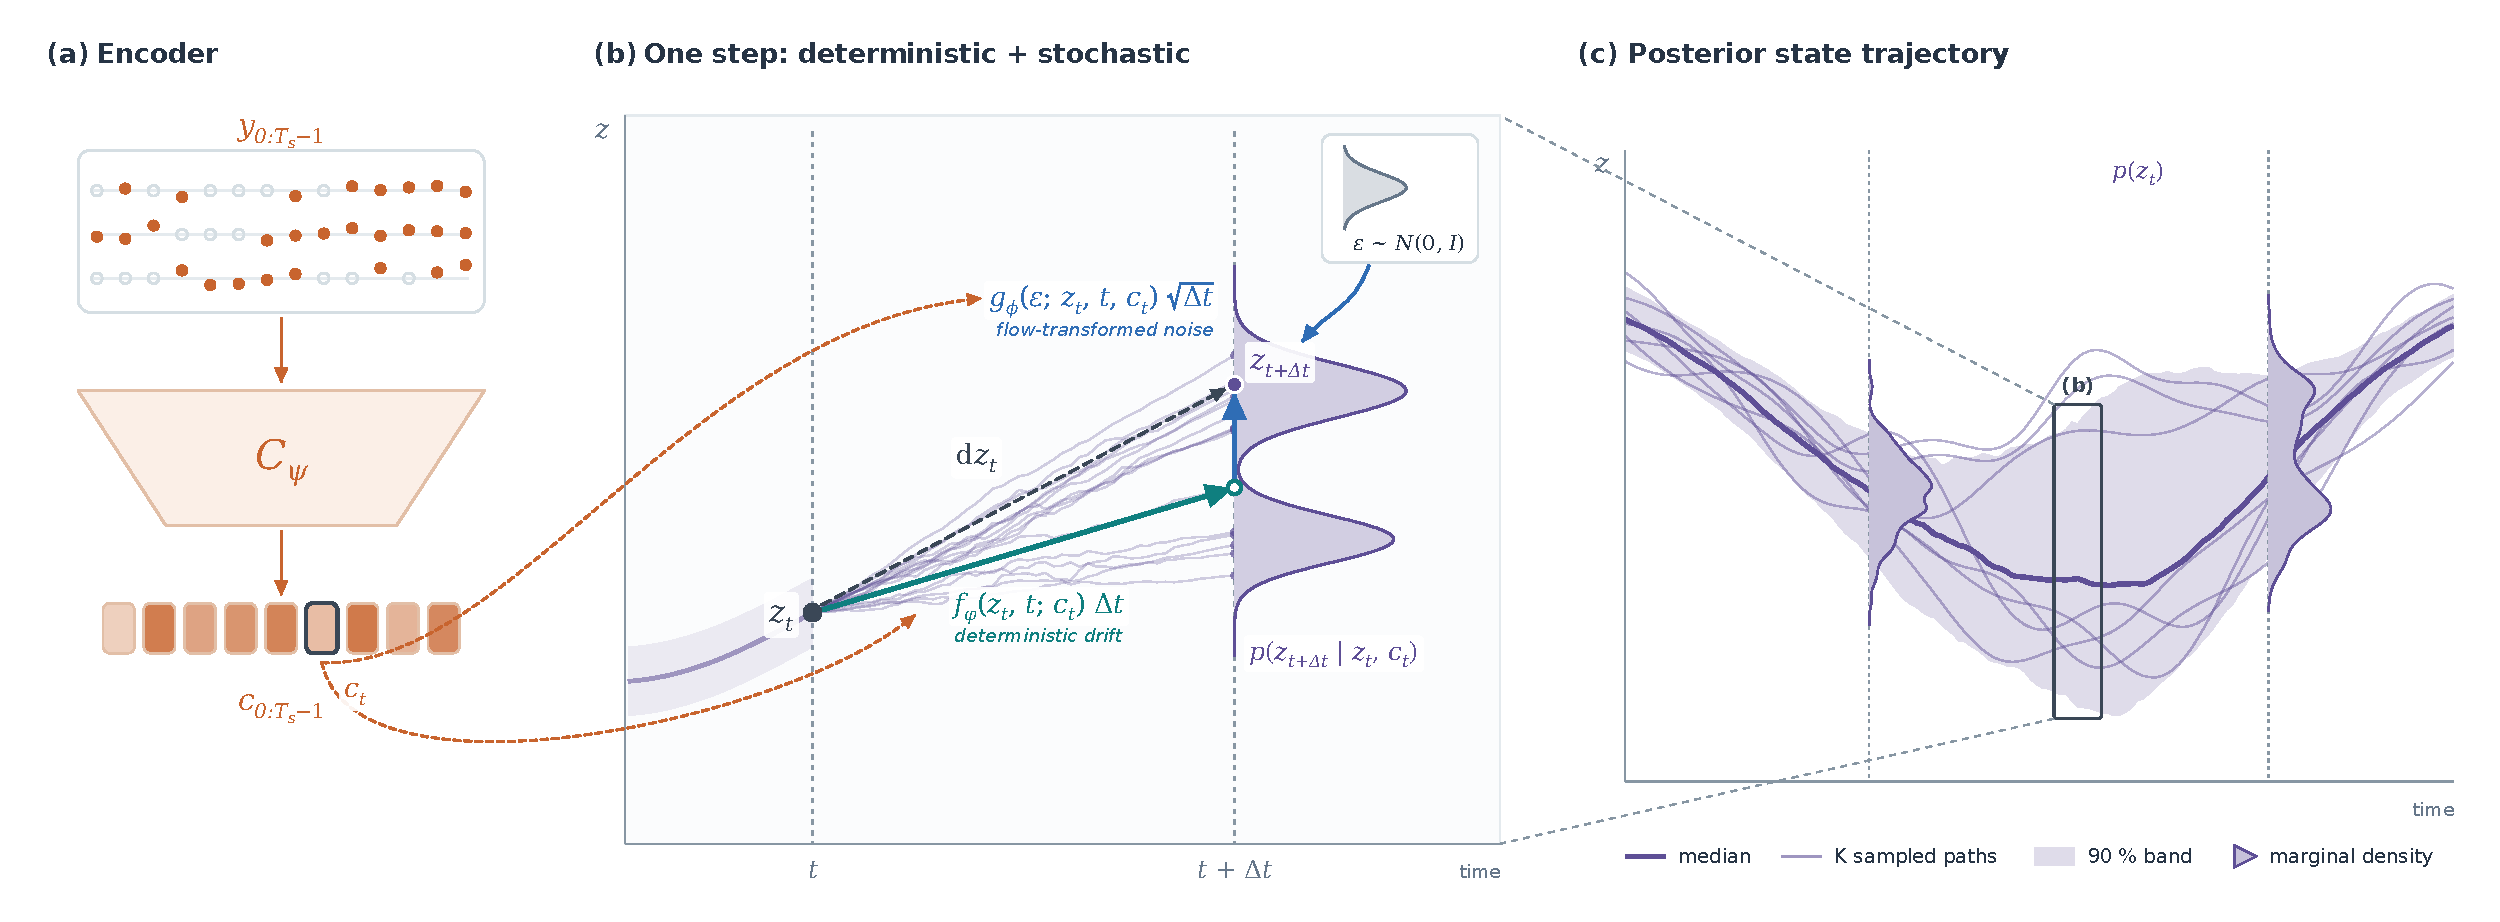
\includegraphics[width=\linewidth]{figures/NormFlowSDE_figure.pdf}
\caption{\method estimates states conditional on observations. (a) At each step, the encoder $C_\psi$ maps a trailing observation window ending before the state being estimated to a context vector $c_t$ (orange), which conditions both the drift and the noise model. The displayed measurement and context arrays summarize these windowwise encodings. (b) Each state update combines a deterministic drift increment (green) with flow-transformed Gaussian noise (blue), yielding a flexible conditional distribution for the next state $z_{t+\Delta t}$ (purple). (c) Repeated updates from the supplied initial state generate $K$ sampled state trajectories; the plot shows their pointwise median, 90\% uncertainty bands, and marginal state densities at selected times. The marginal label $p(z_t)$ leaves the fixed observation windows and controls implicit. The boxed interval is expanded in (b). All curves and densities are schematic.}
\label{fig:overview}
\end{figure}

The construction also raises a mathematical question: under what conditions does the flow-based state update admit a continuous-time SDE limit? In Appendix~\ref{app:diffusion}, we prove that, with the learned coefficients fixed and under explicit regularity and moment assumptions, the trajectories of a centered inference scheme converge in distribution to the unique solution of an It\^o SDE as the time step tends to zero. 

Section~\ref{sec:experiments} evaluates \method as a causal amortized filter on two simulated systems (a controlled pendulum and the Lorenz--96 model) and two robot datasets (ALOHA insertion \citep{zhao2023aloha} and REASSEMBLE \citep{sliwowski2025reassemble}), against three particle filters whose transition and measurement models are learned from the same data: NF-DPF \citep{chen2025flowparticle}, NSF \citep{kiyohara2025nsf}, and FlowSDE \citep{lou2026flowsde}. 

\section{Related Work}\label{sec:related}
For Bayesian state estimation, the relevant question is how a learned model combines temporal dynamics and measurements to represent uncertainty over latent states. Conditional normalizing flows provide samples and tractable densities through change of variables \citep{dinh2014nice,rezende2015flows}. They can approximate an observation-conditioned posterior directly or parameterize the distributions used in a recursive Bayesian filter. We then introduce these three uses through three methods: normalizing flow-based particle filters, Neural Stochastic Flows, and the related flow-matching approach FlowSDE.

\subsection{Normalizing Flows for Amortized Bayesian Inference}
Conditional normalizing flows provide a route to Bayesian inference by learning a distribution over unknown quantities conditioned on observed data. For an unknown parameter vector $\vartheta$ and observations $y$, an invertible map $\vartheta=g_\phi(\epsilon;y)$ transforms a simple base variable $\epsilon\sim\N(0,I)$ into samples from a normalized conditional density $q_\phi(\vartheta\mid y)$, evaluated through change of variables \citep{dinh2014nice,rezende2015flows}. Given training pairs from $p(\vartheta,y)=p(\vartheta)p(y\mid\vartheta)$, conditional maximum likelihood minimizes the expected forward KL divergence from the target posterior to its learned approximation \citep{radev2020bayesflow}:
\begin{equation}\label{eq:amortized-forward-kl}
 \E_{p(\vartheta,y)}[-\log q_\phi(\vartheta\mid y)]
 =\E_{p(y)}\,\left[\KL\,\left(p(\vartheta\mid y)\,\Vert\,q_\phi(\vartheta\mid y)\right)\right]+C_0,
\end{equation}
where $C_0$ is the conditional entropy of $\vartheta$ given the observations, independent of $\phi$. Thus, paired simulations supply a posterior-learning objective without requiring pointwise evaluation of the target posterior.

BayesFlow applies this principle to simulation-based parameter inference, combining a learned summary of the observations with a conditional invertible network \citep{radev2020bayesflow}. Once trained, it produces parameter-posterior samples for new datasets from the same model family without per-dataset optimization. Its inference target is a fixed parameter vector, requiring construction change for an evolving state-inference construction.

Existing temporal extensions illustrate the additional modeling choices. \citet{rasul2021conditionedflows} condition normalizing flows on recurrent or attention-based representations of past observations and covariates, train by conditional likelihood, and generate multivariate forecast trajectories autoregressively. In this formulation, the flow learns a joint distribution between the future states, current states, and past observations, which makes learning extremely difficult and limits the length of the forecast horizon. 

Normalizing Kalman Filters jointly learn an invertible observation transformation and a conditionally linear Gaussian latent state-space model, enabling exact filtering and smoothing in latent space \citep{debezenac2020nkf}. This tractability relies on retaining the linear Gaussian latent structure. Observation-likelihood training alone does not guarantee that the learned latent coordinates correspond to the physical states of interest; using this method for state estimation requires additional structure or state supervision.

\subsection{Particle Filters}
Bayesian filtering updates the distribution of a hidden state as new measurements arrive. A particle filter approximates this distribution, $p(x_k\mid y_{0:k})$, using $M$ candidate states, called particles, and weights describing their relative contributions. The bootstrap particle filter first propagates each previous particle through the transition model by drawing $x_k^{(i)}\sim p(\cdot\mid x_{k-1}^{(i)})$ \citep{gordon1993bootstrap}. These samples represent possible next states before incorporating the new measurement.

The observation likelihood $p(y_k\mid x_k^{(i)})$ then measures how well each predicted state explains the measurement $y_k$. Multiplying the previous weights by these likelihoods and normalizing gives
\begin{equation}\label{eq:bootstrap-weights}
 w_k^{(i)}=
 \frac{w_{k-1}^{(i)}p(y_k\mid x_k^{(i)})}
 {\sum_{j=1}^{M}w_{k-1}^{(j)}p(y_k\mid x_k^{(j)})}.
\end{equation}
Equation~\eqref{eq:bootstrap-weights} is the normalized bootstrap weight update. The numerator combines information from earlier measurements, carried by $w_{k-1}^{(i)}$, with the new evidence; the denominator makes the updated weights sum to one. A standard resampling step can then draw $M$ particles with replacement according to the updated weights and assign the selected particles equal weights $1/M$. Particles with larger weights are more likely to be selected.

Some particle filters use proposals $q$ that incorporate the new measurement. Examples include Gaussian proposals constructed by local linearization \citep{doucet2000sequential} and the unscented particle filter, which constructs a Gaussian proposal for each particle using an unscented Kalman update \citep{vandermerwe2000unscented}. To correct for sampling from such a proposal, each unnormalized weight must also be multiplied by the transition density divided by the proposal density. For the bootstrap filter, the proposal is the transition model itself, so this ratio equals one. Normalizing flows can supply the samples and densities needed to learn these filtering components.

\subsection{Normalizing Flow-Based Differentiable Particle Filters (NF-DPF).}
\citet{chen2025flowparticle} introduce NF-DPF, which learns the transition, proposal, and measurement distributions using three invertible maps. Subscripts $\mathrm{dyn}$, $\mathrm{prop}$, and $\mathrm{obs}$ distinguish their separate parameter sets. With tractable base densities $g_{\theta_{\mathrm{dyn}}}$ and $g_{\theta_{\mathrm{prop}}}$, these models take the form
\begin{equation}\label{eq:nfdpf-components}
\begin{aligned}
 \mathrm{Transition:}\quad x_k^{\mathrm{dyn}}&=f_{\phi_{\mathrm{dyn}}}(\zeta_k^{\mathrm{dyn}}),
 &\zeta_k^{\mathrm{dyn}}&\sim g_{\theta_{\mathrm{dyn}}}(\cdot\mid x_{k-1}),\\
 \mathrm{Proposal:}\quad x_k^{\mathrm{prop}}&=f_{\phi_{\mathrm{prop}}}(\zeta_k^{\mathrm{prop}};y_k),
 &\zeta_k^{\mathrm{prop}}&\sim g_{\theta_{\mathrm{prop}}}(\cdot\mid x_{k-1},y_k),\\
 \mathrm{Measurement:}\quad y_k&=f_{\phi_{\mathrm{obs}}}(\epsilon_k;x_k),
 &\epsilon_k&\sim\N(0,I).
\end{aligned}
\end{equation}
The parameter vectors $\omega_{\mathrm{dyn}}=(\theta_{\mathrm{dyn}},\phi_{\mathrm{dyn}})$ and $\omega_{\mathrm{prop}}=(\theta_{\mathrm{prop}},\phi_{\mathrm{prop}})$ collect the base-density and flow parameters. In Equation~\eqref{eq:nfdpf-components}, the first map defines the transition density $p_{\omega_{\mathrm{dyn}}}(x_k\mid x_{k-1})$. The second defines the proposal $q_{\omega_{\mathrm{prop}}}(x_k\mid x_{k-1},y_k)$, using the measurement to guide candidate generation. These are separate transformations; filtering particles are sampled from the proposal. The third map describes possible observations given a state.

Invertibility makes all three densities evaluable by change of variables. For example, setting $\epsilon_k=f_{\phi_{\mathrm{obs}}}^{-1}(y_k;x_k)$ gives the measurement likelihood
\begin{equation}\label{eq:nfdpf-observation-likelihood}
 p_{\phi_{\mathrm{obs}}}(y_k\mid x_k)
 =p_\epsilon(\epsilon_k)\left|\det\frac{\partial f_{\phi_{\mathrm{obs}}}^{-1}(y_k;x_k)}{\partial y_k}\right|,
\end{equation}
where $p_\epsilon$ is the standard Gaussian density and $x_k$ is held fixed in the Jacobian. For each proposed particle $x_k^{(i)}\sim q_{\omega_{\mathrm{prop}}}(\cdot\mid x_{k-1}^{(i)},y_k)$, these densities enter the update
\begin{equation}\label{eq:nfdpf-weights}
 w_k^{(i)}\propto w_{k-1}^{(i)}
 \frac{\underbrace{p_{\phi_{\mathrm{obs}}}(y_k\mid x_k^{(i)})}_{\mathrm{measurement\ likelihood}}\,
 \underbrace{p_{\omega_{\mathrm{dyn}}}(x_k^{(i)}\mid x_{k-1}^{(i)})}_{\mathrm{transition\ density}}}
 {\underbrace{q_{\omega_{\mathrm{prop}}}(x_k^{(i)}\mid x_{k-1}^{(i)},y_k)}_{\mathrm{proposal\ density}}}.
\end{equation}
The proportionality in Equation~\eqref{eq:nfdpf-weights} leaves normalization implicit: the resulting weights are divided by their sum, as in Equation~\eqref{eq:bootstrap-weights}. The flows supply both candidate states and the density values needed to correct their weights.

NF-DPF uses entropy-regularized optimal-transport resampling to support gradient-based learning. Training maximizes a particle estimate of the observation log likelihood or minimizes supervised state-estimation error. For image observations, an encoder and reconstruction objective are added, and the flow likelihood is evaluated on encoded features. Deployment retains a particle ensemble, likelihood weighting, and resampling, whereas our primary observation-conditioned route directly samples a learned conditional trajectory distribution.

\subsection{Neural Stochastic Flows}
Neural Stochastic Flows (NSFs) use a conditional normalizing flow to model the distribution of a future state $x_t$ given a starting state $x_s$ and a time interval $h=t-s>0$ \citep{kiyohara2025nsf}. The sampling procedure has two stages: a neural network constructs a Gaussian candidate $\widetilde x$, and an invertible network $g_\phi$ transforms that candidate into $x_t$. The context is $a=(x_s,h,s)$, with absolute time $s$ omitted for autonomous dynamics. The two sampling stages are
\begin{equation}\label{eq:nsf-transition-sampling}
\begin{aligned}
 \widetilde x&=x_s+h\mu_\theta(a)+\sqrt h\,\sigma_\theta(a)\odot\epsilon,
 \qquad \epsilon\sim\N(0,I),\\
 x_t&=g_\phi(\widetilde x;a).
\end{aligned}
\end{equation}
Here $\mu_\theta$ and $\sigma_\theta>0$ are outputs of ordinary multilayer perceptrons that set the Gaussian displacement and noise scale; $\odot$ denotes componentwise multiplication. The conditional normalizing flow is $g_\phi$, a composition of invertible affine coupling layers. It acts on the complete candidate state $\widetilde x$, allowing the resulting transition distribution $p_\omega^{s,t}(x_t\mid x_s)$ to be non-Gaussian. Here $\omega=(\theta,\phi)$ collects both the Gaussian-network and flow parameters.

The flow has the composition of $L_{\mathrm f}$ layers: $g_\phi=f_{\phi,L_{\mathrm f}}\circ\cdots\circ f_{\phi,1}$. Each layer splits its input $\zeta$ into coordinate blocks $(\zeta_A,\zeta_B)$ and produces $\zeta'=f_{\phi,\ell}(\zeta;a)$ through
\begin{equation}\label{eq:nsf-affine-coupling}
\begin{aligned}
 \zeta'_A&=\zeta_A,\\
 \zeta'_B&=\zeta_B\odot\exp\,\bigl(h\,\alpha_\ell(\zeta_A,a)\bigr)
       +h\,\beta_\ell(\zeta_A,a).
\end{aligned}
\end{equation}
The networks $\alpha_\ell$ and $\beta_\ell$, whose parameters are included in $\phi$, predict a log scale and a shift from the unchanged block and the context \citep[Section~3.1]{kiyohara2025nsf}. The factors of the time interval $h=t-s$ make every coupling layer the identity at $h=0$, when the Gaussian candidate also reduces to $x_s$. For $h>0$, the inverse transformation and its Jacobian give an evaluable transition density by change of variables. A single pass through the layers samples the state at time $t$ without numerical SDE integration.

Transition densities of a Markov process satisfy the Chapman--Kolmogorov relation: a direct transition must agree with two successive transitions after averaging over the intermediate state \citep[Chapter~4, Section~1]{ethier1986markov}. NSF encourages its learned densities to satisfy this relation:
\begin{equation}\label{eq:nsf-chapman-kolmogorov}
 p_\omega^{s,t}(x_t\mid x_s)
 \approx\int p_\omega^{r,t}(x_t\mid x_r)\,
               p_\omega^{s,r}(x_r\mid x_s)\,dx_r,
 \qquad s<r<t.
\end{equation}
Here $x_r$ is the state at the intermediate time $r$. The exact Markov relation uses equality; the approximation sign indicates that consistency is encouraged rather than guaranteed by NSF.

The integral in Equation~\eqref{eq:nsf-chapman-kolmogorov} is generally intractable. NSF therefore introduces an auxiliary bridge distribution $q_\xi^{\mathrm{br}}(x_r\mid x_s,x_t;s,r,t)$, with trainable parameters $\xi$, to represent plausible intermediate states conditioned on both endpoints \citep{kiyohara2025nsf}. This bridge enables variational upper bounds on the KL divergences between the direct and composed transition distributions in both directions. Averaging the sum of these bounds over sampled time triplets defines the consistency penalty $\mathcal L_{\mathrm{flow}}(\omega,\xi)$.

For observed state pairs $\mathcal D$, training combines this penalty with negative log likelihood:
\begin{equation}\label{eq:nsf-training-objective}
 \mathcal L(\omega,\xi)
 =-\E_{(x_s,x_t,s,t)\sim\mathcal D}
       \log p_\omega^{s,t}(x_t\mid x_s)
   +\lambda\mathcal L_{\mathrm{flow}}(\omega,\xi).
\end{equation}
The first term fits observed transitions, while $\lambda\geq0$ controls the strength of the consistency penalty. The transition parameters $\omega=(\theta,\phi)$ and bridge parameters $\xi$ are learned during training.

The original paper introduces latent NSF for noisy or partially observed sequences, using NSF to model transitions between latent states \citep[Section~4]{kiyohara2025nsf}. In our state-filtering setting, NSF serves as the transition model of a bootstrap particle filter. For comparability, a conditional normalizing flow is used an observation model $q_\psi(y_k\mid x_k)$ and it is trained together by maximum likelihood.

\subsection{FlowSDE}
FlowSDE uses conditional flow matching to train a neural vector field from state-transition data, together with a potential landscape for interpreting critical transitions \citep{lou2026flowsde}. Flow matching specifies how the vector field is trained. The resulting field is used as the drift in the supplementary SDE formulation
\begin{equation}\label{eq:flowsde-related-dynamics}
 dX_t=f_\varphi(X_t,t)\,dt+\sqrt{2D}\,dW_t,
\end{equation}
where $f_\varphi$ is an ordinary neural network that outputs a drift vector, $W_t$ is standard Brownian motion, and $D>0$ is a prescribed scalar diffusion coefficient \citep[Section~1.1]{lou2026flowsde_supp}. The drift describes systematic state changes, while the Brownian term adds random perturbations with covariance $2D I\,dt$.

The flow-matching step constructs supervision for $f_\varphi$ between observed states. The training procedure selects a pair $(x_s,x_t)$ with gap $h=t-s$, chooses an intermediate fraction $\tau\in(0,1)$, and draws a state $\widetilde X_r$ from a Gaussian bridge at physical time $r=s+\tau h$. The chosen bridge supplies an analytic conditional vector-field target $b_r^{\mathrm{br}}$ for the drift network at that state, expressed per unit physical time. Schematically, the data-fitting loss is
\begin{equation}\label{eq:flowsde-cfm-regression}
 \mathcal L_{\mathrm{CFM}}(\theta)
 =\E\,\left[
 \left\|f_\varphi(\widetilde X_r,r)
       -b_r^{\mathrm{br}}(\widetilde X_r\mid x_s,x_t)\right\|^2\right].
\end{equation}
The expectation averages over training pairs, intermediate times, and bridge samples. Each target tells the network the direction and rate of motion to predict at a sampled state. The endpoints determine this training target; the network learns a shared field across pairs. Thus flow matching turns dynamics learning into vector-field regression, without simulating full SDE trajectories or differentiating through a numerical solver during training. Here ``conditional'' refers to the bridge endpoints; observation conditioning is an additional choice in the state-estimation adaptation below. At inference, the learned drift $f_\varphi$ is numerically integrated together with Brownian noise to generate state trajectories. 

A separate network learns a scalar potential $V_\eta$, yielding the decomposition
\begin{equation}\label{eq:flowsde-potential-decomposition}
 f_\varphi(x,t)=-\nabla V_\eta(x)+R_{\theta,\eta}(x,t),
 \qquad R_{\theta,\eta}=f_\varphi+\nabla V_\eta.
\end{equation}
The gradient component points toward lower potential, while the residual permits non-conservative motion, including circulation. The symbol $R_{\theta,\eta}$ denotes this residual force, computed from the drift and potential networks. Potential minima and barriers help interpret stable regions and transitions between them.

The fitting and physical-consistency terms can be summarized as
\begin{equation}\label{eq:flowsde-training-objective}
 \mathcal L(\theta,\eta)
 =\mathcal L_{\mathrm{CFM}}(\theta)
 +\lambda_{\mathrm E}\mathcal L_{\mathrm{EPR}}(\theta,\eta)
 +\lambda_{\mathrm H}\mathcal L_{\mathrm{HJB}}(\theta,\eta)
 +\lambda_{\mathrm O}\mathcal L_{\mathrm{orth}}(\theta,\eta).
\end{equation}
Here $\mathcal L_{\mathrm{CFM}}$ is the vector-field regression in Equation~\eqref{eq:flowsde-cfm-regression}, and the nonnegative $\lambda$ coefficients balance the regularizers. The entropy-production penalty $\mathcal L_{\mathrm{EPR}}$ penalizes the squared residual force under weights derived from $\exp(-V_\eta/D)$. The Hamilton--Jacobi--Bellman penalty $\mathcal L_{\mathrm{HJB}}$ encourages compatibility between the drift and the candidate stationary density $p_{\mathrm{ss}}\propto\exp(-V_\eta/D)$. The orthogonality penalty discourages alignment of $R_{\theta,\eta}$ with $\nabla V_\eta$ \citep[Sections~1.2--1.4]{lou2026flowsde_supp}. These are soft constraints; for time-dependent dynamics, stationary consistency is used as a local regularizer.

As the above two methods, FlowSDE serves as the transition model of a bootstrap particle filter. Its drift is conditioned on state, time, and control input, and particles are propagated by Euler--Maruyama integration of Equation~\eqref{eq:flowsde-related-dynamics}. 

These three methods place learned flows at different points in state inference. NF-DPF learns the transition, proposal, and measurement models of a particle filter. NSF learns finite-interval transition densities and FlowSDE learns a drift by flow matching; in our setting, both serve as transition models of a bootstrap particle filter, so measurements enter only through the weight update. \method instead conditions on encoded measurements and generates states directly, without particle weights or resampling.
\section{NormFlowSDE for Amortized Bayesian State Estimation}\label{sec:method}

\subsection{Observation-Conditioned State Transitions}

To extend conditional normalizing flows to amortized Bayesian state estimation, we represent the state as a time-dependent random variable and combine a conditional flow with the temporal update structure of a neural SDE. A conventional neural SDE has the form
\begin{equation}\label{eq:neural-sde}
 dz_t=f_\varphi(z_t,t,u_t)\,dt+\sigma(z_t,t,u_t)\,dW_t,
\end{equation}
where $z_t\in\R^d$ is the state variable, $u_t$ denotes control inputs, and $W_t$ is a $d$-dimensional Wiener process. The drift $f_\varphi$ determines the infinitesimal conditional mean, while $\sigma\sigma^\top$ determines the conditional covariance per unit time. At physical times $t_k=k\Delta t$, with $\Delta t>0$, the Euler--Maruyama stochastic increment is $\sqrt {\Delta t}\,\sigma(z_k,t_k,u_k)\epsilon_k$, where $\epsilon_k\sim\N(0,I_d)$. We use a fixed physical interval $\Delta t>0$ for training.

For state estimation, $y_k$ denotes the observation at time $t_k$. The encoder uses a window of observations preceding the state being estimated. For an integer window length $o\geq1$, the encoder computes the window feature as
\begin{equation}\label{eq:sequence-conditioning}
 c_k=C_\psi\,\left(y_{\max(0,k-o+1):k}\right),
 \qquad k=0,\ldots,N-1.
\end{equation}
Thus the update to $z_{k+1}$ uses at most the last $o$ observations through $t_k$; near the sequence start, only the available prefix is used. We replace the linear Gaussian noise map with a conditional invertible flow to obtain the finite-step NormFlowSDE update
\begin{equation}\label{eq:normflowsde-overview}
 z_{k+1}=z_k+\Delta t\,f_\varphi(z_k,t_k,u_k,c_k)
          +\sqrt {\Delta t}\,g_\phi(\epsilon_k;z_k,t_k,u_k,c_k),
 \qquad \epsilon_k\stackrel{\mathrm{iid}}\sim\N(0,I_d).
\end{equation}
Here $z_k$ denotes a state sample at time $t_k$, and the Gaussian inputs are independent of the supplied data and initial state. The initial state $z_0$ is provided by the data and initializes the stochastic process once. Each subsequent update uses the current generated state $z_k$, time $t_k$, control $u_k$ when available, and window feature $c_k$.

This construction assigns nominal deterministic evolution to the drift network, while the conditional flow learns the distribution of stochastic increments from data. Both networks receive observation information and reuse their fitted parameters across sequences, enabling amortized conditional trajectory sampling. The flow can also contribute to the conditional mean because its output is uncentered. Appendix~\ref{app:diffusion} constructs a centered inference scheme and proves its weak convergence to an It\^o diffusion under stated assumptions.

We next derive a composite training objective for \method. 

\subsection{Training Objective and Procedure}\label{sec:training}
Training uses paired reference states $x_{0:N}$, observations $y_{0:N-1}$, and controls $u_{0:N-1}$ when available. The reference path $\mathbf x=(x_1,\ldots,x_N)$ supplies supervision, while $\mathbf z=(z_1,\ldots,z_N)$ denotes a generated path. The parameter vector $\omega=(\varphi,\phi,\psi)$ collects all trainable parameters. 

The objective combines reconstruction accuracy, a transition-density term, agreement between training segments, and a distributional score for full trajectories.

\subsubsection{Reconstruction and Transition Terms}
With the supplied initial state, observations, and controls fixed, $q_\omega(\mathbf z)$ denotes the generated path density. We use the Gaussian reconstruction model $p_\sigma(x_k\mid z_k)=\N(x_k;z_k,\sigma_{\mathrm{state}}^2I_d)$, where the fixed scale $\sigma_{\mathrm{state}}>0$ weights state errors. The reconstruction and transition losses are
\begin{align}
 \mathcal L_{\mathrm{state}}(\omega;\mathbf x)
 &=\frac{1}{2\sigma_{\mathrm{state}}^2}
   \E_{\mathbf z\sim q_\omega}
   \left[\sum_{k=1}^N\norm{x_k-z_k}^2\right]
   +\frac{Nd}{2}\log(2\pi\sigma_{\mathrm{state}}^2),\label{eq:state-training-loss}\\
 \mathcal L_{\mathrm{trans}}(\omega)
 &=\E_{\mathbf z\sim q_\omega}[-\log q_\omega(\mathbf z)]
   =H(q_\omega),\label{eq:transition-training-loss}
\end{align}
where $H(q_\omega)$ is the differential entropy of the generated path. The reconstruction scale is distinct from observation noise and learned transition uncertainty.

Both expectations are taken over generated paths, which are not available in closed form: evaluating $\mathcal L_{\mathrm{state}}$ requires integrating Equation~\eqref{eq:normflowsde-overview} forward from the supplied initial state, one step per physical interval, with a fresh Gaussian input at every step. Equation~\eqref{eq:normflowsde-overview} is itself an Euler--Maruyama-type update \citep{kloeden1992numerical}, and this is the sampler we use by default. Higher-order stochastic solvers can be applied with adaptation of the stochastic term, such as Heun \citep{rumelin1982numerical,kloeden1992numerical}, reversible Heun \citet{kidger2021efficient}, midpoint  \citep{milstein2004stochastic} solvers.

For a differentiable, invertible flow with nonsingular forward Jacobian $J_{\phi,k}(\epsilon)=\partial g_\phi(\epsilon;z_k,t_k,u_k,c_k)/\partial\epsilon$, change of variables in Equation~\eqref{eq:normflowsde-overview} gives
\begin{equation}\label{eq:sampled-transition-density}
 \log q_\omega(z_{k+1}\mid z_k,t_k,u_k,c_k)
 =\log\N(\epsilon_k;0,I_d)
  -\log|\det J_{\phi,k}(\epsilon_k)|-\frac d2\log\Delta t.
\end{equation}
The Gaussian log density has a parameter-independent expectation because $\epsilon_k\sim\N(0,I_d)$. Thus only the expected sum of forward log determinants in $\mathcal L_{\mathrm{trans}}$ affects optimization.

Minimizing this entropy term favors concentrated transitions. To keep the transitions nondegenerate, the RealNVP coupling log scales are bounded in $(-\alpha,\alpha)$. For a flow with $L_{\mathrm f}$ coupling layers, where layer $\ell$ rescales $d_\ell$ coordinates, this bounds the Jacobian determinant on both sides:
\begin{equation}\label{eq:training-determinant-bound}
 e^{-B}\leq|\det J_{\phi,k}(\epsilon)|\leq e^B,
 \qquad B=\alpha\sum_{\ell=1}^{L_{\mathrm f}} d_\ell,
 \qquad \epsilon\in\R^d.
\end{equation}
The lower side bounds the transition entropy below, so the entropy term cannot collapse the stochastic increments. As a side effect, it also imposes a noise floor that is set by $\alpha$ and $L_{\mathrm f}$. Thus, a learnable per-coordinate factor is required. We multiply the bounded flow $T_\phi$ by a learned scale,
\begin{equation}\label{eq:learned-noise-scale}
 g_\phi(\epsilon;z_k,t_k,u_k,c_k)
 =\mathrm{diag}\bigl(s_\phi(z_k,t_k,u_k,c_k)\bigr)\,T_\phi(\epsilon;z_k,t_k,u_k,c_k),
\end{equation}
which is bounded within a much wider range and initialized to one.

The sum $\mathcal L_{\mathrm{state}}+\mathcal L_{\mathrm{trans}}$ builds a composite reconstruction-and-entropy objective. Appendix~\ref{app:training-loss} gives the derivation, the determinant and entropy bounds.

\subsubsection{Multiple Shooting and Boundary Consistency}
To shorten the trajectories through which gradients must be propagated, we choose an integer segment length $L_S\geq2$, counted in state points. This count includes the supplied initial state, so each full segment advances $L_S-1$ time steps and ends at local index $k=L_S-1$. We divide the $N$ transitions into $S$ segments, including a shorter final segment when needed:
\begin{equation}\label{eq:segment-partition}
 S=\left\lceil\frac{N}{L_S-1}\right\rceil,\qquad
 \sum_{s=1}^S(L^{(s)}-1)=N,\qquad
 L^{(s)}=1+\min\{L_S-1,\,N-(s-1)(L_S-1)\},\qquad s=1,\ldots,S.
\end{equation}
Here $s$ labels the segment and $L^{(s)}$ is its actual number of state points. Local index $k$ in segment $s$ corresponds to global time index $(s-1)(L_S-1)+k$.

The supplied initial state of each segment initializes its training rollout. We generate the segments independently in parallel, with the same parameters $\omega$. The boundary penalty compares the predicted endpoint of each nonfinal segment at $k=L_S-1$ with the next supplied initial state at $k=0$:
\begin{equation}\label{eq:continuity-training-loss}
 \mathcal L_{\mathrm{cont}}(\omega)
 =\E
 \left[\sum_{s=1}^{S-1}\norm{z_{L_S-1}^{(s)}-z_0^{(s+1)}}^2\right].
\end{equation}
The expectation is estimated by averaging the summed squared boundary discrepancies over sampled segment rollouts.

\subsubsection{Full-Horizon Distributional Supervision}\label{sec:training-rollout}
To account for errors that accumulate over the complete horizon, we generate full trajectories from the supplied initial state $z_0$, without restarting at segment boundaries. The vectors $\mathbf z$ and $\mathbf z'$ denote two such trajectories generated using independent Gaussian inputs, with the same observations, controls, and initial state. We compare them with the reference trajectory $\mathbf x$ using the energy score \citep{gneiting2007proper}:
\begin{equation}\label{eq:flow_sde_rollout_loss}
 \mathcal L_{\mathrm{rollout}}(\omega;\mathbf x)
 =\E\,\left[\norm{\mathbf z-\mathbf x}\right]
 -\frac12\E\,\left[\norm{\mathbf z-\mathbf z'}\right].
\end{equation}
Each norm is the unsquared Euclidean distance over all time steps and state coordinates. The expectations average over the generated trajectories, holding the supplied data fixed. The first term encourages agreement with the reference trajectory. The second rewards separation between generated trajectories and counteracts their collapse to a single prediction.

During training, we generate $M\geq2$ independent full trajectories $\mathbf z^{(1)},\ldots,\mathbf z^{(M)}$ and compute
\begin{equation}\label{eq:energy-score-estimator}
 \widehat{\mathcal L}_{\mathrm{rollout}}(\omega;\mathbf x)
 =\frac1M\sum_{i=1}^M\norm{\mathbf z^{(i)}-\mathbf x}
 -\frac{1}{2M(M-1)}\sum_{i\ne j}\norm{\mathbf z^{(i)}-\mathbf z^{(j)}}.
\end{equation}
This estimator averages distances to the reference and subtracts half the average distance between distinct generated trajectories. The second sum includes both orders of each pair and excludes self-pairs, giving an unbiased estimate of Equation~\eqref{eq:flow_sde_rollout_loss}.

For fixed observations, controls, and initial state, the expected energy score over reference trajectories is uniquely minimized by matching their true conditional distribution, provided the reference and generated trajectories have finite expected norms \citep{gneiting2007proper,szekely2013energy}. The energy score helps maintain diversity among generated samples while encouraging agreement with the reference trajectory.

\subsubsection{Combined Objective and Optimization}
The combined training objective is
\begin{equation}\label{eq:normflowsde_loss}
 \E_{\mathcal D_{\mathrm{train}}}
 [\mathcal L(\omega;\mathbf x)] = \E_{\mathcal D_{\mathrm{train}}}
 [\mathcal L_{\mathrm{state}}(\omega;\mathbf x)
 +\mathcal L_{\mathrm{trans}}(\omega)+\lambda_{\mathrm{cont}}\mathcal L_{\mathrm{cont}}(\omega)
 +\lambda_{\mathrm{rollout}}\mathcal L_{\mathrm{rollout}}(\omega;\mathbf x)].
 \end{equation}
Here $\E_{\mathcal D_{\mathrm{train}}}$ averages over paired reference states, raw observations, controls, and supplied initial states, together with the selected segment partitions and anchors. We evaluate the rollout term every five optimizer updates to reduce the computational cost. 

% Placeholder for numbers that are filled in once the benchmark is frozen.
\providecommand{\tbd}{\textbf{[TBD]}}
\providecommand{\figplaceholder}[1]{\fbox{\parbox[c][0.28\linewidth][c]{0.96\linewidth}{\centering\small Figure placeholder: #1}}}

\section{Empirical evaluation}\label{sec:experiments}
We evaluate \method as a causal amortized Bayesian filter on two simulated systems and two robot datasets, and compare it with three particle-filter baselines that learn their transition and measurement models from the same data. All four datasets are observed through the same heavy-tailed, multimodal measurement noise, so that the comparison also tests how each method copes with a non-Gaussian likelihood. We evaluate the accuracy of the filtering distributions, the calibration of their uncertainty intervals, the sensitivity to the noise model, and the inference cost. All methods have the same information access, use the same data splits and update budgets, and are scored with the same metrics. Every number in this section is produced from the frozen run directories by the scripts listed in Appendix~\ref{app:reproducibility}.

\subsection{Datasets}\label{sec:experiments-data}
Table~\ref{tab:datasets} summarizes the four datasets. Each sequence consists of a known initial state, a control sequence, and noisy observations of the subsequent states. The reference states are used only for training and scoring. Every dataset is split by trajectory or episode before windowing, and normalization statistics are computed on the training split only.

\paragraph{Observation noise.}
Each observed coordinate is corrupted independently by the same three-component Gaussian mixture,
\begin{equation}\label{eq:obsnoise}
 V\sim 0.70\,\N\!\big(0,(0.5\sigma)^2\big)+0.15\,\N\!\big(2.5\sigma,(1.5\sigma)^2\big)+0.15\,\N\!\big(-2.5\sigma,(1.5\sigma)^2\big),
\end{equation}
whose scale $\sigma$ is 0.1 for the pendulum (in rad and rad/s), 0.5 for Lorenz--96, and 0.1 in normalized units for the two robot datasets. The mixture has standard deviation $1.65\,\sigma$. The Gaussian with the same mean and variance has total-variation distance 0.332 to this mixture and this number is a reference point for Section~\ref{sec:experiments-noise}.

\begin{table}[t]
\centering\footnotesize
\begin{tabular}{lllll}
\toprule
 & Pendulum & Lorenz--96 & ALOHA insertion & REASSEMBLE \\
\midrule
Source & simulated & simulated & sim.\ demonstrations & real robot \\
State dimension $d$ & 2 & 12 & 14 & 7 \\
Observed coordinates & 2 & 6 & 14 & 7 \\
Control dimension & 1 & -- & 14 & 9 \\
Observation noise & mixture, $\sigma=0.1$ & mixture, $\sigma=0.5$ & mixture, $\sigma=0.1$ & mixture, $\sigma=0.1$ \\
Time step $\Delta t$ & 0.05 & 0.02 & 0.02 & 1/30 \\
Window length (steps) & 60 & 100 & 250 & 250 \\
Train / val.\ / test windows & 224 / 48 / 48 & 1600 / 200 / 100 & 400 / 50 / 50 & 2000 / 300 / 300 \\
Samples / particles $M$ & 128 & 200 & 200 & 500 \\
Metric units & physical & physical & normalized & normalized \\
\bottomrule
\end{tabular}
\caption{Datasets. The observation noise is the mixture of Equation~\eqref{eq:obsnoise} with the stated scale $\sigma$; ``sim.\ demonstrations'' refers to human teleoperation recorded in simulation. $M$ is the number of posterior draws scored per window (Appendix~\ref{app:protocol}).}
\label{tab:datasets}
\end{table}

\paragraph{Controlled pendulum.}
A damped pendulum driven by a scalar torque $u$, simulated as the It\^o SDE
\begin{equation}\label{eq:pendulum}
 d\theta=\omega\,dt+\sigma_\theta\,dW_\theta,\qquad
 d\omega=\Big(\frac{u}{m\ell^{2}}-c\,\omega-\frac{g}{\ell}\sin\theta\Big)dt+\sigma_\omega\,dW_\omega,
\end{equation}
with $g=9.81$, $\ell=m=1$, damping $c=0.2$, and process-noise scales $\sigma_\theta=0.01$ and $\sigma_\omega=0.2$, integrated by Euler--Maruyama with eight substeps per observation interval $\Delta t=0.05$. The initial state is known to every filter and drawn as $\theta_0\sim\mathrm{U}(-\pi,\pi)$, $\omega_0\sim\N(0,0.6^{2})$. Both coordinates are observed. 

\paragraph{Lorenz--96.}
The twelve-dimensional Lorenz--96 system,
\begin{equation}\label{eq:lorenz96}
 \frac{dx_i}{dt}=(x_{i+1}-x_{i-2})x_{i-1}-x_i+F,
 \qquad i=0,\ldots,11,\qquad F=8,
\end{equation}
with cyclic indices, integrated with a fourth-order Runge--Kutta scheme at $\Delta t=0.02$. Each window is an independent trajectory: its initial state is drawn as $x(0)\sim\N(0,\,0.01^{2}I)$, integrated for a spin-up of 500 steps so that it lies on the attractor, and the state at the end of the spin-up is the known initial state $x_0$ of the window. Only every second coordinate is observed, so six coordinates must be inferred from the dynamics alone. 

\paragraph{ALOHA insertion.}
Bimanual peg-insertion demonstrations from the ALOHA simulation benchmark, recorded by human teleoperation at 50\,Hz \citep{zhao2023aloha}. Each frame stores two different 14-dimensional joint vectors, which we keep apart: the \emph{commanded} joint positions (the leader-arm targets sent to the position controllers of the follower arms) serve as the control input, and the \emph{measured} joint positions of the follower arms define the state. The two differ by the tracking error of the controllers, which is largest during contact. The recorded states are deterministic given the commands, so we perturb them by a slowly varying latent disturbance (a four-dimensional AR(1) velocity offset whose magnitude grows with the tracking error, that is, during contact) before normalization. The exact recipe is given in Appendix~\ref{app:reproducibility}. The perturbed trajectory is the reference state, and it is observed through the noise of Equation~\eqref{eq:obsnoise} with $\sigma=0.1$ in normalized units. 

\paragraph{REASSEMBLE.}
Contact-rich assembly and disassembly episodes recorded on a real seven-degree-of-freedom robot arm at 30\,Hz \citep{sliwowski2025reassemble}. The state consists of the seven joint positions and all states are obesrvable. The nine-dimensional robot commands serve as controls. Unlike the other datasets, the dynamics are those of a physical system interacting with its environment, and no model of them is available.

\subsection{Compared Methods}\label{sec:experiments-methods}
All four methods are causal Bayesian filters: the estimate of $x_{k+1}$ uses the observations up to and including $y_{k+1}$, starts from the known initial state. NF-DPF, NSF, and FlowSDE are used in particle filters, which obtain their uncertainty from the observations through Bayesian weighting with learned transition and measurement models. NF-DPF also learns an observation-conditioned proposal, whereas NSF and FlowSDE run as bootstrap filters. \method infers the state distribution directly from the observations. For the two simulated systems, pendulum and Lorenz--96, we also report model-based reference filters that use the true dynamics and the true noise scale: an extended Kalman filter (EKF) and an unscented Kalman filter (UKF) with the moment-matched Gaussian likelihood, and a bootstrap particle filter with the exact mixture likelihood. These references indicate the accuracy attainable with perfect models and are not competitors.

\subsection{Benchmark Results}\label{sec:experiments-results}
Table~\ref{tab:main-results} compares the four methods on four datasets. Each configuration is trained with three independent seeds, and we report the mean and standard deviation over seeds. Accuracy is measured by the RMSE of the posterior mean, averaged over test windows. Distributional accuracy is measured by the continuous ranked probability score (CRPS) and the energy score \citep{gneiting2007proper}, averaged over coordinates. Calibration is measured by the empirical coverage of central 90\% marginal intervals, pooled over windows, steps and coordinates, which is read together with their mean width. Inference cost is the median wall-clock time to filter one test window on a single GPU.

\begin{table}[htbp]
\centering\footnotesize
\resizebox{\linewidth}{!}{%
\begin{tabular}{llccccc}
\toprule
Dataset & Method & RMSE $\downarrow$ & CRPS $\downarrow$ & Cov.\ 90\% & Width & Latency (ms) $\downarrow$ \\
\midrule
Pendulum & \method & 0.0691 $\pm$ 0.0008 & 0.0362 $\pm$ 0.0004 & 0.834 $\pm$ 0.017 & 0.1862 $\pm$ 0.0093 & \textbf{6.7} \\
 & NF-DPF & \textbf{0.0629 $\pm$ 0.0007} & \textbf{0.0320 $\pm$ 0.0003} & \textbf{0.918 $\pm$ 0.006} & 0.2017 $\pm$ 0.0017 & 14.5 \\
 & NSF & 0.0687 $\pm$ 0.0029 & 0.0346 $\pm$ 0.0014 & 0.866 $\pm$ 0.035 & 0.1805 $\pm$ 0.0110 & 12.6 \\
 & FlowSDE & 0.1144 $\pm$ 0.0069 & 0.0578 $\pm$ 0.0026 & 0.918 $\pm$ 0.003 & 0.3107 $\pm$ 0.0012 & 16.2 \\
 & EKF / UKF & 0.0578 $\pm$ 0.0000 & 0.0296 $\pm$ 0.0000 & 0.870 $\pm$ 0.001 & 0.1650 $\pm$ 0.0002 & 12.3 / 12.2 \\
 & bootstrap PF & 0.0406 $\pm$ 0.0003 & 0.0192 $\pm$ 0.0001 & 0.895 $\pm$ 0.002 & 0.1129 $\pm$ 0.0000 & 10.4 \\
\midrule
Lorenz--96 & \method & 0.2942 $\pm$ 0.0082 & 0.1586 $\pm$ 0.0040 & 0.880 $\pm$ 0.016 & 0.8715 $\pm$ 0.0394 & \textbf{14.2} \\
 & NF-DPF & 0.2899 $\pm$ 0.0086 & 0.1585 $\pm$ 0.0051 & 0.854 $\pm$ 0.022 & 0.7811 $\pm$ 0.0645 & 30.9 \\
 & NSF & \textbf{0.2290 $\pm$ 0.0173} & \textbf{0.1199 $\pm$ 0.0103} & 0.822 $\pm$ 0.019 & 0.4692 $\pm$ 0.0053 & 20.6 \\
 & FlowSDE & 0.3227 $\pm$ 0.0067 & 0.1749 $\pm$ 0.0043 & \textbf{0.890 $\pm$ 0.009} & 0.9554 $\pm$ 0.0412 & 33.4 \\
 & EKF / UKF & 0.0229 $\pm$ 0.0000 & 0.0093 $\pm$ 0.0000 & 0.997 $\pm$ 0.000 & 0.0906 $\pm$ 0.0001 & 12.7 / 19.0 \\
 & bootstrap PF & 0.0188 $\pm$ 0.0001 & 0.0077 $\pm$ 0.0000 & 0.990 $\pm$ 0.000 & 0.0674 $\pm$ 0.0000 & 15.4 \\
\midrule
ALOHA & \method & \textbf{0.0538 $\pm$ 0.0011} & \textbf{0.0301 $\pm$ 0.0007} & \textbf{0.871 $\pm$ 0.013} & 0.1645 $\pm$ 0.0017 & \textbf{19.5} \\
 & NF-DPF & 0.1307 $\pm$ 0.0288 & 0.0780 $\pm$ 0.0186 & 0.658 $\pm$ 0.065 & 0.2278 $\pm$ 0.0031 & 49.7 \\
 & NSF & 0.0858 $\pm$ 0.0006 & 0.0501 $\pm$ 0.0004 & 0.821 $\pm$ 0.005 & 0.2339 $\pm$ 0.0012 & 37.8 \\
 & FlowSDE & 0.0717 $\pm$ 0.0004 & 0.0413 $\pm$ 0.0002 & 0.858 $\pm$ 0.006 & 0.2147 $\pm$ 0.0047 & 49.4 \\
\midrule
REASSEMBLE & \method & \textbf{0.0326 $\pm$ 0.0016} & \textbf{0.0179 $\pm$ 0.0008} & \textbf{0.903 $\pm$ 0.005} & 0.1026 $\pm$ 0.0022 & \textbf{21.4} \\
 & NF-DPF & 0.0613 $\pm$ 0.0006 & 0.0340 $\pm$ 0.0003 & 0.858 $\pm$ 0.004 & 0.1760 $\pm$ 0.0021 & 47.8 \\
 & NSF & 0.0615 $\pm$ 0.0002 & 0.0345 $\pm$ 0.0001 & 0.916 $\pm$ 0.000 & 0.2140 $\pm$ 0.0003 & 43.0 \\
 & FlowSDE & 0.0530 $\pm$ 0.0012 & 0.0300 $\pm$ 0.0007 & 0.951 $\pm$ 0.001 & 0.2136 $\pm$ 0.0045 & 57.3 \\
\bottomrule
\end{tabular}
}
\caption{Test results, mean $\pm$ standard deviation over three training seeds, with $M$ posterior draws per window as in Table~\ref{tab:datasets} and, for the particle filters, the particle count of the dataset protocol (500, 1000, 200, 500). RMSE and width are in the metric units of Table~\ref{tab:datasets}. Coverage is nominally 0.90. Latency is the median time in milliseconds to filter one test window in the configuration of the row (seed 0, one NVIDIA L40S, compilation excluded). For the EKF / UKF, latency is measured with the same protocol.}
\label{tab:main-results}
\end{table}

\paragraph{Robot datasets.}
On ALOHA and REASSEMBLE, \method attains the lowest RMSE and CRPS by a wide margin, with the narrowest intervals and a coverage close to the nominal level (0.87 and 0.90). Here the transition dynamics are high-dimensional, and for REASSEMBLE they are those of a physical, contact-rich system. The particle filters rely on a learned one-step transition model and a learned measurement density, and errors in either directly affect their weights. NF-DPF in particular loses accuracy and coverage on ALOHA. \method instead learns the observation-conditioned update directly and uses every observed coordinate without an explicit likelihood.

\paragraph{Simulated systems.}
On the pendulum and Lorenz--96, particle filters with learned models are more accurate than \method: NF-DPF reaches the lowest RMSE on the pendulum and NSF on Lorenz--96. Both systems have smooth, low-dimensional dynamics that a one-step transition model can learn accurately from clean state pairs, and once these models are accurate, Bayesian weighting is close to optimal. The reference filters put the numbers in perspective. On the pendulum, the exact-likelihood particle filter with the true model reaches 0.041, whereas the Gaussian filters with the true dynamics but the moment-matched likelihood (EKF, UKF) reach only 0.058 and a coverage of 0.87: three quarters of the gap between the best learned filter and the model-based filters is caused by the noise model alone, a point we return to in Section~\ref{sec:experiments-noise}. On Lorenz--96 the reference particle filter reaches 0.019, an order of magnitude below every learned method, but it owes this to the exact chaotic dynamics. The learned methods, at 0.23 to 0.32, therefore operate at the accuracy of a dynamics model with a few percent error, which the chaotic flow amplifies over the window, and the six unobserved coordinates can only be inferred through that model. NSF, the most accurate learned method on Lorenz--96 but at a much more under-covered level (0.82).

\paragraph{Calibration.}
Figure~\ref{fig:calibration} shows the empirical coverage of central intervals at nominal levels from 10\% to 95\%. \method lies on the diagonal on Lorenz--96, ALOHA and REASSEMBLE at every level (within 0.03, 0.04 and 0.05 of the nominal level, respectively), so its intervals are calibrated as a whole and not only at 90\%. On the pendulum it is under-dispersed at every level by about one tenth (0.45 at the 50\% level, 0.83 at 90\%). The shortfall is concentrated in the angle coordinate during the first steps after the known initial state, where the predictive spread grows more slowly than the error (angle coverage 0.80 against 0.87 for the velocity, and 0.62 over the first five steps). The particle filters are miscalibrated in both directions depending on the dataset: NF-DPF is over-dispersed on the pendulum (0.56 at the 50\% level) and strongly under-dispersed on ALOHA (0.33 at 50\%, 0.66 at 90\%). FlowSDE is over-dispersed on the pendulum and REASSEMBLE (0.63 at 50\%). NSF is under-dispersed at the high levels on Lorenz--96 and ALOHA (0.82 at 90\%). At equal accuracy \method's intervals are also the narrowest (Table~\ref{tab:main-results}: 0.16 against 0.21--0.23 on ALOHA, 0.10 against 0.18--0.21 on REASSEMBLE). The reference filters are over-dispersed on Lorenz--96 (coverage 0.99 at the 90\% level with the validation-selected process noise), so even the true model does not yield calibrated intervals on the chaotic system.

\begin{figure}[htbp]
\centering
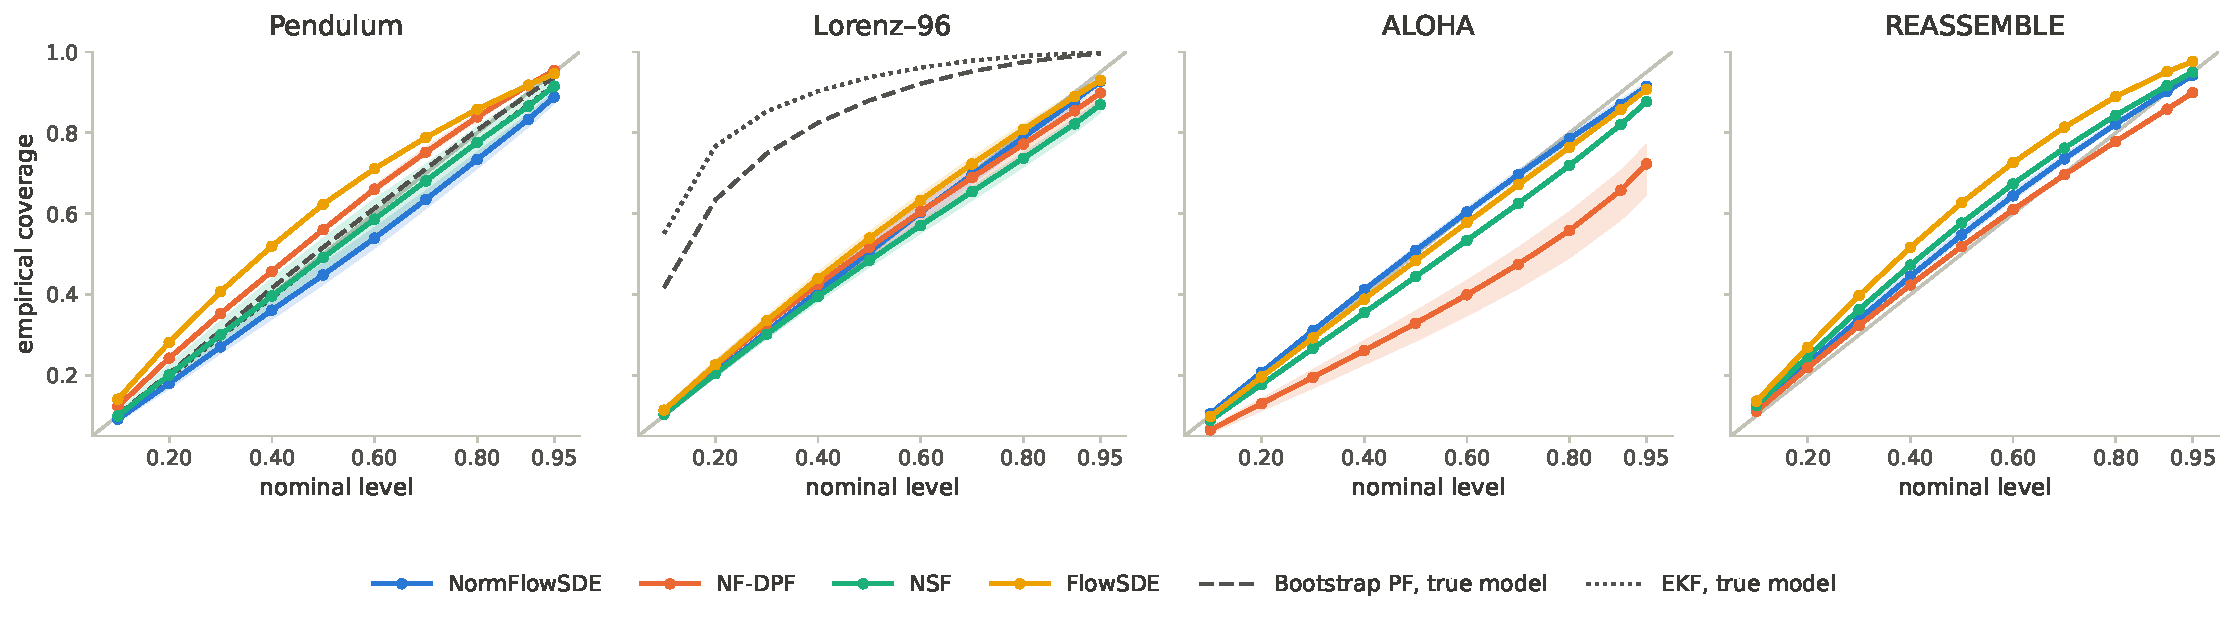
\includegraphics[width=\linewidth]{figures/calibration.pdf}
\caption{Calibration of central marginal intervals at nominal levels from 10\% to 95\%, pooled over test windows, steps, and coordinates (mean over three seeds; shaded: range over seeds). The diagonal indicates perfect calibration. Gray curves: reference filters with the true model on the simulated systems.}
\label{fig:calibration}
\end{figure}

\paragraph{Latency.}
A \method sample requires one network evaluation per time step, without weighting or resampling. A particle filter additionally evaluates the measurement density for every particle at every step and resamples when the effective sample size drops. The latency column of Table~\ref{tab:main-results} reports the median time to filter one test window in the configuration of each row. \method is the fastest method on every dataset, by a factor of 1.5 to 2.0 over the fastest particle filter and 2.3 to 2.7 over the slowest. The advantage is largest on the two robot datasets, where the 14- and 7-dimensional measurement densities are the most expensive part of the particle filters.

\subsection{Observation-Noise Recovery}\label{sec:experiments-noise}
The mixture noise of Equation~\eqref{eq:obsnoise} is the main difference between this benchmark and the usual Gaussian setting. The reference filters in Table~\ref{tab:main-results} already show its price for a method with the wrong noise model: with the true dynamics, the Gaussian filters lose a third of their accuracy on the pendulum relative to the exact-likelihood particle filter (0.058 against 0.041). We therefore investigate wether the learned method actually recover the noise distribution from data.

\begin{figure}[t]
\centering
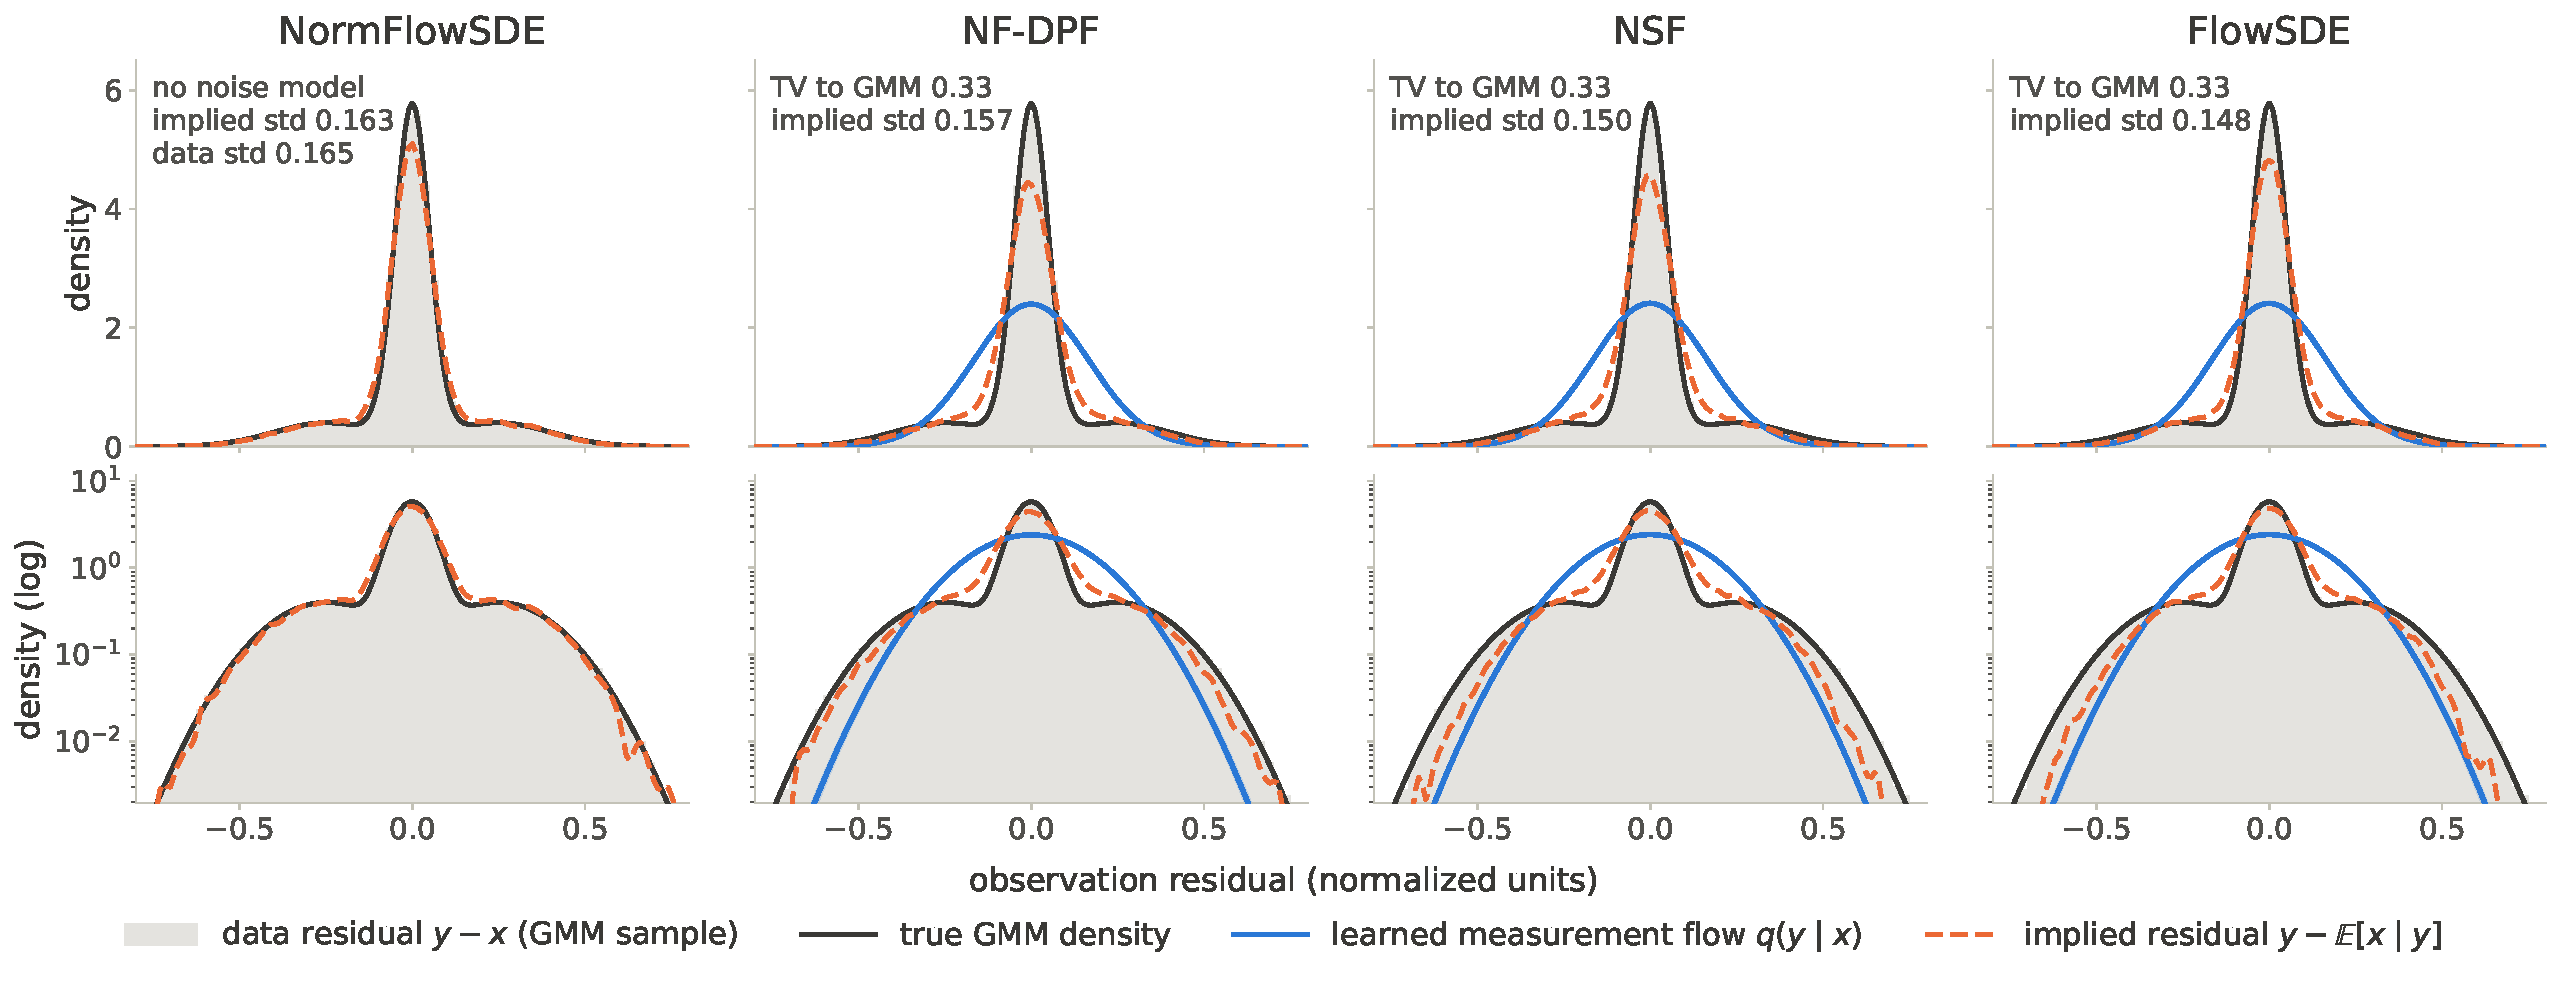
\includegraphics[width=\linewidth]{figures/measurement_density_reassemble.pdf}
\caption{Recovery of the observation noise on REASSEMBLE (seed 0, normalized units). Gray: histogram of the data residuals $y-x$; black: the mixture of Equation~\eqref{eq:obsnoise}; blue: the learned measurement flow $q(y\mid x)$ of each particle filter, averaged over 100 test states and all coordinates (band: 10th to 90th percentile over states); orange, dashed: the implied residuals $y-\E[x\mid y]$ of each method's posterior mean. Top: linear scale; bottom: logarithmic scale. The three learned flows coincide with the moment-matched Gaussian (total variation 0.33 to the mixture, analytic value 0.332), whereas the implied residuals of \method follow the mixture.}
\label{fig:noise-recovery}
\end{figure}

Figure~\ref{fig:noise-recovery} compares the learned measurement densities with the true mixture on REASSEMBLE. For the three particle filters we evaluate the learned conditional flow $q(y\mid x)$ along one-coordinate slices $y=x+\delta e_j$ around test states and average over states and coordinates. \method has no measurement model. For every method we show the distribution of the implied residuals $y-\E[x\mid y]$, which means the observations minus the posterior mean. The result is the same for all three particle filters: the learned measurement flows match the variance of the noise but none of its shape. Their total-variation distance to the mixture is 0.33, which equals the analytic distance (0.332) between the mixture and its moment-matched Gaussian. This indicates the flows have converged to the moment-matched Gaussian. 

Three consequences follow. (i) The learned particle filters weight their particles with a Gaussian likelihood on mixture data: too little weight on particles that agree with a measurement from the sharp central component, too little tolerance for the side modes. They therefore inherit the deficit of the EKF and UKF in Table~\ref{tab:main-results}. (ii) Three flows with different architectures and training signals stop at the same density on every dataset. A conditional affine coupling flow on a Gaussian base, fitted by maximum likelihood, has little incentive to move beyond the second moment when the heavy tails appear in only a few percent of the training pairs. (iii) \method recovers the noise structure implicitly. Its implied residuals reproduce the mixture over four decades of density on every dataset, including central spike and side modes with a standard deviation within 4\% of the data. Trained on the rollout objective alone, the amortized update has learned how much to trust each measurement: one from the sharp central component is highly informative, whereas one from a side mode is much less so. This is exactly the information that a correct likelihood encodes. The implied residuals of the particle filters are sharper than their learned likelihoods, because resampling with the dynamics partly corrects the wrong weights. But the residual spread of NSF and FlowSDE is 7\% to 10\% below the data: their posterior means follow the noisy measurements rather than the state.

\subsection{Summary}\label{sec:experiments-summary}
\method is the most accurate filter on both robot datasets, is calibrated at all nominal levels on three of the four datasets, and is the fastest method on every dataset. On the two simulated systems, particle filters with accurately learned dynamics are more accurate. This advantage stems from their importance weighting. However, the noise-recovery analysis shows the price of that weighting: the learned measurement densities of all three particle filters collapse to the moment-matched Gaussian, so they weight their particles with the wrong likelihood, whereas the amortized update of \method reproduces the mixture implicitly. \method is therefore most attractive when the dynamics are complex or physical and hard to model explicitly, when the measurement noise is not Gaussian, and when fast and calibrated inference is required.

\section{Discussion and limitations}\label{sec:discussion}
\paragraph{Benchmark}
The four methods differ in one design decision: whether the observation enters the estimate through a likelihood and importance weights, or through a learned update that is trained end to end on complete filtering rollouts. The benchmark separates the two regimes cleanly. When the dynamics are simple enough to learn from clean state pairs, weighting achieves higher accuracy: on the pendulum and Lorenz--96 the best learned particle filter is 9\% and 22\% more accurate than \method. The model-based filters show that the remaining gap to perfect inference is small on the pendulum and dominated by chaotic error amplification on Lorenz--96. When the dynamics are complex (such ascontact-rich) and not governed by a closed-form model, as on the two robot datasets, the learned update excels by a wide margin (25\% and 38\% lower RMSE on ALOHA and REASSEMBLE), with calibrated intervals and about half the latency. The reason is that the filtering distribution of \method is trained on the scored quantity over the whole window, which reduces the modeling errors of the transition and observation models.

\paragraph{The likelihood is the weak point of learned particle filters.}
The noise-recovery analysis (Section~\ref{sec:experiments-noise}) shows all three learned measurement densities converge to the moment-matched Gaussian of the true mixture noise. Maximum-likelihood training of conditional normalizing flows causes the underfitting of the heavy tails, and only the variance is matched instead. \method applies additional energy-score objective contributes to a precise fit of the implied residuals. 

\paragraph{Coverage.}
Coverage probability of an amortized filter relies entirely on the training objective. Two terms are essential: the learned per-coordinate noise scale enabling arbitrary noise scales, and an energy-score based rollout term ensuring proper calibration. Where this balance holds, the intervals are calibrated at every nominal level (Figure~\ref{fig:calibration}). 

\paragraph{Limitations.}
\method is under-covered on the pendulum (0.83 at the 90\% level), mainly in the angle coordinate during the first steps after the known initial state. The learned noise scale and the energy-score term calibrate the other three datasets but do not guarantee calibration. Partially observed chaotic dynamics remain difficult: on Lorenz--96 the six unobserved coordinates can be inferred only through the dynamics, and without a transition model and importance weights \method reaches 0.29 against 0.019 for the reference particle filter. Training also requires careful tuning. The objective of Equation~\eqref{eq:normflowsde_loss} balances four terms, and coverage is sensitive to the rollout weight $\lambda_{\mathrm{rollout}}$, the state scale $\sigma_{\mathrm{state}}$, and the initial noise scale. These were selected on validation trajectories separately for each dataset, and a new system requires the same search.

\section{Conclusion}
\method replaces the likelihood and importance weights of a particle filter by an observation-conditioned normalizing-flow update that is trained end to end on complete filtering rollouts. The benchmark of four datasets with heavy-tailed, multimodal measurement noise shows what this design buys and what it costs. On the two robot datasets it is the most accurate filter with calibrated intervals that are also the narrowest. Because one sample costs one network evaluation per step, without per-particle likelihoods or resampling, it is the fastest method on every dataset, at 1.5 to 2 times the speed of the fastest particle filter. It is also the only learned method whose implied residuals recover the mixture noise, whereas the learned likelihoods of all three particle filters collapse to a Gaussian. The price is paid on simple simulated dynamics, where a learned transition model combined with Bayesian weighting is more accurate, most clearly under partial observation of the chaotic Lorenz--96 system. These results argue for amortized filtering wherever the dynamics are hard to model, the noise is not Gaussian, and inference must be fast and calibrated, and they identify the learned measurement likelihood as the component of particle filters most in need of a better training objective.
\bibliography{references}
\bibliographystyle{tmlr}
\clearpage
\appendix
\section{Weak convergence of the centered NormFlowSDE inference scheme}
\label{app:diffusion}\label{sec:weak_conv_norm_flowsde}

This appendix gives the full argument behind the continuous-time interpretation in Section~\ref{sec:method}. The starting point is the trained, finite-step transition. We first construct an inference scheme that preserves that transition at its training interval, then prove convergence of its trajectories as the inference step decreases. The result concerns a conditional generative model; it does not identify its coefficients with the physical dynamics of the observed system.

\subsection{What is held fixed, and why the noise must be centered}

Write $h_0=\Delta t_{\mathrm{train}}>0$ for the physical interval of the trained transition and $h=\Delta t_{\mathrm{inf}}>0$ for the inference step. Fix a finite time horizon $[0,T]$ and a deterministic, continuous schedule $\xi=(u(\cdot),c(\cdot))$ of controls and observation features. The fitted parameters, training step $h_0$, and schedule $\xi$ remain fixed throughout; only the inference step $h$ tends to zero. Any step-size inputs to the networks are held at their training values. The initial state $z_0\in\R^d$ is supplied by the data and is also fixed. Every inference chain and the limiting process start from this same value, $Z_0^h=Z_0=z_0$. Conditioning on $z_0$ is implicit in all probabilities and expectations below. We retain the schedule in every coefficient, with
\begin{align*}
 f_\varphi(z,t;\xi)&:=f_\varphi(z,t,u(t),c(t)),\\
 g_\phi(\epsilon;z,t,\xi)&:=g_\phi(\epsilon;z,t,u(t),c(t)).
\end{align*}
The resulting coefficients must satisfy the stated assumptions for this fixed $\xi$; the constants below may depend on $\xi$. At each trained time $t_k$, $c(t_k)$ is the feature computed from the preceding observation window defined in Section~\ref{sec:method}. 

We use $z\in\R^d$ for a fixed state value and $Z$ for a random state. At time $t$, the trained update is
\begin{equation}\label{eq:trainingupdate}
 \begin{aligned}
 Z'&=z+h_0 f_\varphi(z,t;\xi)+\sqrt{h_0}\,g_\phi(\epsilon;z,t,\xi),\\
 \epsilon\mid z,t,\xi&\sim\N(0,I_d).
 \end{aligned}
\end{equation}
where $f_\varphi$ is the drift network and $g_\phi$ is the conditional flow. Assume its conditional mean exists, and define
\begin{align}\label{eq:centerednoise}
 m_\phi(z,t;\xi)&=\E_\epsilon[g_\phi(\epsilon;z,t,\xi)],\\
 \eta_c(z,t,\epsilon;\xi)&=g_\phi(\epsilon;z,t,\xi)-m_\phi(z,t;\xi).\notag
\end{align}
Here and below, $\E_\epsilon$ denotes integration over $\epsilon\sim\N(0,I_d)$ with the displayed state, time, and schedule fixed. Thus $\E_\epsilon[\eta_c(z,t,\epsilon;\xi)]=0$. The effective drift of the trained transition is its expected increment per unit time:
\begin{equation}\label{eq:effectivedrift}
 b_{\mathrm{eff}}(z,t;\xi)
 =f_\varphi(z,t;\xi)+\frac{m_\phi(z,t;\xi)}{\sqrt{h_0}}
 =\frac{\E[Z'-z\mid z,t,\xi]}{h_0}.
\end{equation}
Using this drift and the centered noise gives the inference map 
\begin{equation}\label{eq:refinement}
 F_{h,t}(z,\epsilon;\xi)
 =z+h b_{\mathrm{eff}}(z,t;\xi)+\sqrt h\,\eta_c(z,t,\epsilon;\xi).
\end{equation}
We distinguish the fixed training step $h_0$ from the inference step $h$ to preserve the learned transition at $h=h_0$. Centering the stochastic increment and compensating the drift then avoid a divergent mean contribution as $h\to0$.


\subsection{The limiting process and sufficient assumptions}\label{sec:limit-statement}

Repeated application of the inference map in Equation~\eqref{eq:refinement}, at times $t_k=kh$, gives
\begin{equation}\label{eq:centered}
 Z^h_{k+1}=Z^h_k+h b_{\mathrm{eff}}(Z^h_k,t_k;\xi)
                 +\sqrt h\,\eta_c(Z^h_k,t_k,\epsilon_k;\xi).
\end{equation}
For a current state $z$, the increment has conditional mean $h b_{\mathrm{eff}}(z,t;\xi)$ and covariance $hA(z,t;\xi)$, where
\begin{equation}\label{eq:limitcovariance}
 A(z,t;\xi)=\E_\epsilon[\eta_c(z,t,\epsilon;\xi)\eta_c(z,t,\epsilon;\xi)^\top].
\end{equation}
This identifies the candidate diffusion: its drift is $b_{\mathrm{eff}}$ and its diffusion covariance is $A$. Write its noise coefficient as a matrix $\sigma$ satisfying $\sigma\sigma^\top=A$. The conditions below ensure that matching these local moments also leads to convergence of complete trajectories.

\begin{assumption}[Conditions for diffusion convergence]\label{ass:limit}
On the finite horizon $[0,T]$, assume the following.
\begin{enumerate}
\item \textnormal{\bfseries Regular drift and diffusion.}\label{ass:limit-regularity}
The functions $b_{\mathrm{eff}}(z,t;\xi)$ and a covariance factor $\sigma(z,t;\xi)$ with $\sigma\sigma^\top=A$ are jointly continuous in $(z,t)$, globally Lipschitz in $z$, and of at most linear growth in $z$. The Lipschitz and growth constants are uniform in $t\in[0,T]$. These conditions control the trajectories and ensure uniqueness of the limiting SDE.
\item \textnormal{\bfseries Controlled noise moments.}\label{ass:limit-moments}
The centered noise $\eta_c$ is jointly measurable, and its third moment is bounded on every bounded state region, uniformly in time:
\begin{equation}\label{eq:local-third-assumption}
 \sup_{\norm z\leq R,\,t\in[0,T]}
 \E_\epsilon\norm{\eta_c(z,t,\epsilon;\xi)}^3<\infty,
 \qquad R<\infty.
\end{equation}
This condition controls the Taylor approximation error and the probability of large increments.
\item \textnormal{\bfseries Given initial state and independent noise.}\label{ass:limit-initial}
Every chain starts at the data-provided state $Z_0^h=z_0$. With $z_0$ and $\xi$ fixed, the Gaussian inputs $\epsilon_k\sim\N(0,I_d)$ are independent across steps. Thus trajectory randomness comes from the generated increments, not from sampling an initial state.
\end{enumerate}
\end{assumption}

\begin{theorem}[Weak convergence of the centered inference scheme]\label{thm:weak}
Under Assumption~\ref{ass:limit}, the paths generated by Equation~\eqref{eq:centered}, held constant between grid points as $\bar Z^h_t=Z^h_{\lfloor t/h\rfloor}$, satisfy
\[
 \operatorname{Law}(\bar Z^h\mid\xi)
 \Longrightarrow\operatorname{Law}(Z\mid\xi)
 \qquad(h\to0),
\]
in $D([0,T],\R^d)$ with the Skorokhod $J_1$ topology. The limit $Z$ is the unique-in-law solution of
\begin{equation}\label{eq:limit}
 \begin{aligned}
 dZ_t&=b_{\mathrm{eff}}(Z_t,t;\xi)\,dt+\sigma(Z_t,t;\xi)\,dW_t,\\
 Z_0&=z_0.
 \end{aligned}
\end{equation}
Conditional on the fixed data, $W$ is a standard $d$-dimensional Brownian motion. For every three-times continuously differentiable test function $v$ with compact support, the discrete generators also converge uniformly on bounded state regions and $t\in[0,T]$, as specified in Equation~\eqref{eq:generator} below.
\end{theorem}

The theorem compares distributions of whole trajectories. The space $D([0,T],\R^d)$ contains right-continuous paths with left limits, including the piecewise-constant paths $\bar Z^h$. Its Skorokhod $J_1$ topology allows small shifts in jump times when comparing paths \citep{skorokhod1956limit}; the limiting SDE paths are continuous. Section~\ref{sec:consistency-proof} now shows how the three assumptions turn the local moment match into this path-convergence result.

\subsection{Proof of Theorem~\ref{thm:weak}}\label{sec:consistency-proof}
The proof has two tasks: show that the trajectory distributions have limits, and identify those limits. Step~1 calculates the expected change over one inference step. Steps~2--4 then control whole trajectories: they prevent escape to arbitrarily large states, remove persistent jumps, and bound changes over short time intervals. Step~5 shows that any resulting limit must have the law of the SDE in Equation~\eqref{eq:limit}. We use the standard diffusion-approximation result of \citet{ethier1986markov,kushner2001numerical} to connect the path estimates and the limiting expected-change identity.

\paragraph{1. Identify the local diffusion limit.}
For a scalar test function $v\in C_c^3(\R^d)$, meaning that $v$ has three continuous derivatives and compact support, define
\begin{equation}\label{eq:discretegenerator}
 \mathcal L_{h,t}^{\xi}v(z)
 =\frac{\E_\epsilon[v(F_{h,t}(z,\epsilon;\xi))]-v(z)}h.
\end{equation}
This is the expected change of $v$ in one inference step, divided by the step duration. To calculate its limit, fix $(z,t,\xi)$ and write
$\Delta=h b_{\mathrm{eff}}(z,t;\xi)+\sqrt h\,\eta_c(z,t,\epsilon;\xi)$.
Throughout this local calculation, the arguments $(z,t,\xi)$ are held fixed and suppressed on $b_{\mathrm{eff}}$, $\eta_c$, and $A$:
\begin{align}\label{eq:proofmoments}
 \E[\Delta\mid z,t,\xi]
 &=h b_{\mathrm{eff}}+\sqrt h\,\E_\epsilon[\eta_c]
 =h b_{\mathrm{eff}},\notag\\
 \E[\Delta\Delta^\top\mid z,t,\xi]
 &=h^2b_{\mathrm{eff}}b_{\mathrm{eff}}^\top
   +h\E_\epsilon[\eta_c\eta_c^\top]+h^{3/2}\bigl(
 b_{\mathrm{eff}}\E_\epsilon[\eta_c]^\top
 +\E_\epsilon[\eta_c]b_{\mathrm{eff}}^\top\bigr)\notag\\
 &=h^2b_{\mathrm{eff}}b_{\mathrm{eff}}^\top+hA.
\end{align}
The $h^{3/2}$ line displays both drift--noise cross terms. They vanish because the noise is centered, $\E_\epsilon[\eta_c]=0$. The remaining noise term is its covariance $A$, defined in Equation~\eqref{eq:limitcovariance}.

Taylor's formula gives
\begin{equation}\label{eq:taylorexpansion}
 v(z+\Delta)-v(z)
 =\nabla v(z)^\top\Delta
  +\tfrac12\Delta^\top\nabla^2v(z)\Delta+R_v(z,\Delta),
 \qquad |R_v(z,\Delta)|\leq C_v\norm\Delta^3.
\end{equation}
Here $\nabla v$ and $\nabla^2v$ are the gradient and Hessian. To control the remainder, we need the \emph{third absolute moment of the full increment} $\Delta$. The drift is bounded on each region $\norm z\leq R$, $t\in[0,T]$, and the noise third moment is bounded by Equation~\eqref{eq:local-third-assumption}. Hence, for $0<h\leq1$,
\begin{align}\label{eq:thirdmoment}
 \E[\norm\Delta^3\mid z,t,\xi]
 &\leq4h^3\norm{b_{\mathrm{eff}}(z,t;\xi)}^3
   +4h^{3/2}\E_\epsilon\norm{\eta_c(z,t,\epsilon;\xi)}^3\notag\\
 &\leq C_{R,T}h^{3/2},
 \qquad \norm z\leq R,\quad t\in[0,T].
\end{align}
The constant is independent of $h$, $z$, and $t$ within this region. It is derived from, and distinct from, the assumed noise-moment bound.

Substituting the moments from Equation~\eqref{eq:proofmoments} into the expected Taylor expansion gives the full generator calculation:
\begin{align}\label{eq:generator-error}
 \mathcal L_{h,t}^{\xi}v(z)
 &=\frac1h\left(
 \nabla v(z)^\top\E_\epsilon\Delta
 +\frac12\operatorname{tr}\,\left(\nabla^2v(z)\E_\epsilon[\Delta\Delta^\top]\right)
 +\E_\epsilon R_v(z,\Delta)\right)\notag\\
 &=\frac1h\left(
 h\nabla v(z)^\top b_{\mathrm{eff}}
 +\frac12\operatorname{tr}\,\left(\nabla^2v(z)
       [hA+h^2b_{\mathrm{eff}}b_{\mathrm{eff}}^\top]\right)
 +\E_\epsilon R_v(z,\Delta)\right)\notag\\
 &=b_{\mathrm{eff}}^\top\nabla v(z)
   +\frac12\operatorname{tr}\,\left(A\nabla^2v(z)\right)
   +\frac h2 b_{\mathrm{eff}}^\top\nabla^2v(z)b_{\mathrm{eff}}
   +\frac{\E_\epsilon R_v(z,\Delta)}h .
\end{align}
The last two terms vanish uniformly on each bounded state region, since
\begin{align}\label{eq:generator-remainder}
 &\sup_{\norm z\leq R,\,t\in[0,T]}
 \left|\frac h2 b_{\mathrm{eff}}^\top\nabla^2v(z)b_{\mathrm{eff}}
       +\frac{\E_\epsilon R_v(z,\Delta)}h\right|\notag\\
 &\quad\leq
 \frac h2\sup_{\norm z\leq R,\,t\in[0,T]}
       \bigl(\norm{b_{\mathrm{eff}}}^2\norm{\nabla^2v(z)}_{\mathrm{op}}\bigr)
 +\frac{C_v}h\sup_{\norm z\leq R,\,t\in[0,T]}\E_\epsilon\norm\Delta^3
 \leq C_{R,T,v}(h+\sqrt h)\longrightarrow0.
\end{align}
Here $\norm{\cdot}_{\mathrm{op}}$ is the matrix operator norm. Thus the limiting generator is
\begin{equation}\label{eq:generator}
 \mathcal L_t^{\xi}v(z)
 =\lim_{h\to0}\mathcal L_{h,t}^{\xi}v(z)
 \overset{\mathrm{(\ref{eq:discretegenerator}),\,(\ref{eq:refinement})}}{=}
 \lim_{h\to0}\frac{
 \E_\epsilon[v(F_{h,t}(z,\epsilon;\xi))-v(z)]}{h}.
\end{equation}
Equations~\eqref{eq:generator-error}--\eqref{eq:generator-remainder} identify this limiting expected change with the drift and covariance terms of the candidate SDE. This proves the local conclusion of Theorem~\ref{thm:weak}; the remaining steps concern entire paths.

\paragraph{2. Bound the probability of leaving a large state region.}
The local calculation above is uniform only when the state stays in a bounded region. For a radius $R>\norm{z_0}$, we use the closed Euclidean ball centered at the origin,
\begin{equation}\label{eq:state-ball}
 \overline B(0,R):=\{z\in\R^d:\norm z\leq R\}.
\end{equation}
Here $\norm{\cdot}$ is the Euclidean norm, so the ball contains every state whose distance from the origin is at most $R$, including its boundary. We need to show that paths are unlikely to leave this ball over the entire time horizon, with a bound that does not deteriorate as $h$ decreases. We set $N_h=\lfloor T/h\rfloor$ and use the notation
\[
 b_k=b_{\mathrm{eff}}(Z_k^h,t_k;\xi),\qquad
 A_k=A(Z_k^h,t_k;\xi),\qquad
 \eta_k=\eta_c(Z_k^h,t_k,\epsilon_k;\xi).
\]
The linear-growth assumption gives
\begin{equation}\label{eq:innovation-growth}
 \norm{b_{\mathrm{eff}}(z,t;\xi)}^2+
 \E_\epsilon\norm{\eta_c(z,t,\epsilon;\xi)}^2
 =\norm{b_{\mathrm{eff}}(z,t;\xi)}^2+\operatorname{tr}A(z,t;\xi)
 \leq C(1+\norm z^2).
\end{equation}
We measure the size of a state by $V(z)=1+\norm z^2$. Centering and the growth bound imply, for $0<h\leq1$,
\begin{align}\label{eq:one-step-size}
 \E[V(Z_{k+1}^h)\mid Z^h_{0:k},\xi]
 &=1+\norm{Z_k^h+h b_k}^2+h\operatorname{tr}A_k\notag\\
 &\leq1+(1+h)\norm{Z_k^h}^2+(h+h^2)\norm{b_k}^2
          +h\operatorname{tr}A_k\notag\\
 &\leq(1+Ch)V(Z_k^h).
\end{align}
Here $Z^h_{0:k}$ denotes the generated history through step $k$. The bound says that the expected squared size grows by a factor at most $1+Ch$ per step.

To turn this into a bound for the whole path, we freeze a copy of the chain at its first exit from $\overline B(0,R)$. Exit from this closed ball means $\norm{Z_k^h}>R$:
\[
 \tau_R=\inf\{k\leq N_h:\norm{Z_k^h}>R\},\qquad
 Y_k^h=Z^h_{\min(k,\tau_R)},\qquad \inf\varnothing=\infty.
\]
This stopped copy is only a proof device; it does not change the inference algorithm. Before exit it follows the original chain, including the step that crosses the boundary. After exit it stays at that exit state. Equation~\eqref{eq:one-step-size} therefore also bounds its expected size, and iteration gives
\begin{align}\label{eq:stopped-size}
 \E[V(Y_{k+1}^h)\mid Z^h_{0:k},\xi]
 &\leq(1+Ch)V(Y_k^h),\notag\\
 \E[V(Y_{N_h}^h)\mid\xi]
 &\leq(1+Ch)^{N_h}V(z_0)
 \leq e^{CT}(1+\norm{z_0}^2)=:C_T.
\end{align}
If any state leaves the ball, the frozen final state has squared norm greater than $R^2$. Hence
\begin{equation}\label{eq:containment}
 \Pr\,\left(\max_{k\leq N_h}\norm{Z_k^h}>R\,\middle|\,\xi\right)
 =\Pr(\tau_R\leq N_h\mid\xi)
 \leq\frac{\E[V(Y_{N_h}^h)\mid\xi]}{1+R^2}
 \leq\frac{C_T}{1+R^2}.
\end{equation}
The same bound applies to $\sup_{t\leq T}\norm{\bar Z_t^h}$. For any probability tolerance $\varepsilon>0$, we can choose $R$ large enough that $C_T/(1+R^2)\leq\varepsilon$. This single radius works for every $0<h\leq1$: the process $\bar Z^h$ remains in $\overline B(0,R)$ throughout $[0,T]$ with probability at least $1-\varepsilon$. Because closed bounded balls in $\R^d$ are compact, this is the \emph{compact containment condition} of \citet[Chapter~3, Remark~7.3, p.~129]{ethier1986markov}.

\paragraph{3. Combine the one-step and whole-path jump bounds.}
Fix a jump threshold $a>0$. Equation~\eqref{eq:thirdmoment} bounds the third absolute moment of the full increment. Since $\norm\Delta^2\leq\norm\Delta^3/a$ whenever $\norm\Delta>a$,
\begin{equation}\label{eq:smalljumps}
 \sup_{\norm z\leq R,\,t\in[0,T]}
 \frac1h\E[\norm\Delta^2\boldsymbol 1_{\{\norm\Delta>a\}}\mid z,t,\xi]
 \qquad\leq\frac1{ah}
 \sup_{\norm z\leq R,\,t\in[0,T]}\E[\norm\Delta^3\mid z,t,\xi]
 \leq\frac{C_{R,T}}a\sqrt h\longrightarrow0.
\end{equation}
The indicator selects increments larger than $a$. This proves that large increments contribute vanishing second moment per unit time.

We also need the probability of encountering even one large jump along the path. The same third-moment estimate bounds each such probability by $C_{R,T}h^{3/2}/a^3$ while the starting state is inside the ball. There are at most $T/h$ increments. Adding these probabilities and the escape probability from Step~2 gives
\begin{align}\label{eq:maximum-jump}
 \Pr\,\left(\max_{k<N_h}\norm{Z_{k+1}^h-Z_k^h}>a\,\middle|\,\xi\right)
 &\quad\leq\Pr(\tau_R\leq N_h\mid\xi)
 +\sum_{k<N_h}\Pr\,\left(\norm{Z_{k+1}^h-Z_k^h}>a,\quad k<\tau_R\,\middle|\,\xi\right)\notag\\
 &\quad\leq\frac{C_T}{1+R^2}+\frac{T}{h}\frac{C_{R,T}h^{3/2}}{a^3}
 =\frac{C_T}{1+R^2}+\frac{T C_{R,T}}{a^3}\sqrt h .
\end{align}
First choose $R$ large, then let $h$ decrease. The largest jump over the whole horizon tends to zero in probability.

\paragraph{4. Bound the change over a short time interval.}
Small individual jumps do not rule out many small increments adding up rapidly. For example, continuous paths $x_n(t)=\sin(nt)$ stay bounded and have no jumps, yet change by order one over intervals of length $1/n$. 

Start at a grid index $K\leq N_h$ that may be chosen from the generated history, such as the first threshold crossing, capped at $N_h$. The choice cannot use future noise: whether $K\leq k$ must be determined at step $k$. Look ahead a fixed number $m$ of steps, ending at $L=\min(K+m,N_h)$; their duration is at most $\ell=mh$. We first bound the change of the stopped copy $Y^h$ from Step~2, so every active update starts inside the ball. Set
\[
 B_R=\sup_{\norm z\leq R,\,t\in[0,T]}\norm{b_{\mathrm{eff}}(z,t;\xi)},
 \qquad
 D_R=\sup_{\norm z\leq R,\,t\in[0,T]}\operatorname{tr}A(z,t;\xi).
\]
Both constants are finite. Let $I_j$ equal one when $K\leq j<L$ and $j<\tau_R$, and zero otherwise. There are at most $m$ active steps, so $\sum_j I_j\leq m$. The increment splits into accumulated drift and noise:
\begin{equation}\label{eq:interval-decomposition}
 Y_L^h-Y_K^h
 =\underbrace{\sum_{j<N_h}I_j h b_j}_{D_{K,m}^h}
  +\underbrace{\sum_{j<N_h}I_j\sqrt h\,\eta_j}_{M_{K,m}^h}.
\end{equation}
Each $I_j$ is determined before $\epsilon_j$ is drawn. Thus the active noise increments still have zero conditional mean, and cross terms between different noise increments vanish. Consequently,
\begin{align}\label{eq:interval-components}
 \norm{D_{K,m}^h}^2
 &\leq\left(\sum_{j<N_h}I_jh B_R\right)^2
 \leq B_R^2\ell^2,\notag\\
 \E[\norm{M_{K,m}^h}^2\mid\xi]
 &=\E\,\left[\sum_{j<N_h}I_jh\operatorname{tr}A_j\,\middle|\,\xi\right]
 \leq D_R\ell.
\end{align}
The drift grows with elapsed time; the noise \emph{variance} grows with elapsed time. We do not assume that the accumulated drift and noise are independent. Using $\norm{D+M}^2\leq2\norm D^2+2\norm M^2$ gives
\begin{equation}\label{eq:short-increment}
 \E[\norm{Y_L^h-Y_K^h}^2\mid\xi]
 \leq2B_R^2\ell^2+2D_R\ell.
\end{equation}
Except when the original path exits the ball, its increment equals that of the stopped copy. For $\ell\leq\delta+h$,
\begin{align}\label{eq:short-increment-probability}
 \Pr(\norm{Z_L^h-Z_K^h}>a\mid\xi)
 &\leq\Pr(\tau_R\leq N_h\mid\xi)
    +\frac{\E[\norm{Y_L^h-Y_K^h}^2\mid\xi]}{a^2}\notag\\
 &\leq\frac{C_T}{1+R^2}
   +\frac{2}{a^2}\left[B_R^2(\delta+h)^2+D_R(\delta+h)\right].
\end{align}
Choose $R$ large first. With that radius fixed, the second term tends to zero as the interval length $\delta$ and step $h$ decrease. Thus a large change is unlikely over a short interval, even when its starting time is selected from the generated history.

For starting times between grid points, rounding to the grid alters the compared increment by at most two grid jumps; Step~3 shows that this error vanishes. The containment and short-interval estimates are the compactness conditions in the cited diffusion-approximation result: every sequence $h\to0$ has a subsequence whose path laws converge. This property is called \emph{tightness}. Together with the vanishing jumps, these bounds ensure that the possible limits have continuous paths.

\paragraph{5. Identify the limit through its expected changes.}
Steps~2--4 establish the existence of subsequential limits, but do not yet specify their law. Let $X$ denote any such limit. We now show why its law must be that of the SDE in Equation~\eqref{eq:limit}.

\emph{From one step to an interval.}
The generator predicts the expected change of any smooth test function $v$:
\begin{equation}\label{eq:conditional-test-increment}
 \E[v(Z^h_{j+1})-v(Z^h_j)-h\mathcal L_{h,t_j}^{\xi}v(Z_j^h)
       \mid Z^h_{0:j},\xi]=0.
\end{equation}
Thus \emph{actual change minus predicted change} has zero conditional mean. For grid indices $p<q$, sum these differences for the stopped copy from Step~2. The state changes telescope, giving
\begin{equation}\label{eq:stopped-expected-change}
 \E\,\left[
 \underbrace{v(Y_q^h)-v(Y_p^h)}_{\mbox{\scriptsize actual change}}
 -\underbrace{\sum_{j=p}^{q-1}\boldsymbol 1_{\{j<\tau_R\}}
       h\mathcal L_{h,t_j}^{\xi}v(Z_j^h)}_{\mbox{\scriptsize accumulated predicted change}}
 \,\middle|\,Z^h_{0:p},\xi\right]=0.
\end{equation}
Stopping ensures that every rate in this sum is evaluated inside the region where Step~1 gives uniform convergence.

\emph{From the discrete sum to a time integral.}
Replacing each discrete rate by $\mathcal L_{t_j}^{\xi}v$ incurs a total error bounded by
\[
 \left|\sum_{j=p}^{q-1}\boldsymbol 1_{\{j<\tau_R\}}h
  \bigl(\mathcal L_{h,t_j}^{\xi}v-\mathcal L_{t_j}^{\xi}v\bigr)(Z_j^h)\right|
 \leq T\sup_{\norm z\leq R,\,t\in[0,T]}
       |\mathcal L_{h,t}^{\xi}v(z)-\mathcal L_t^{\xi}v(z)|
 \longrightarrow0.
\]
Continuity of the limiting paths and coefficients turns the sum of limiting rates into its time integral. The cited diffusion-approximation result passes the stopped conditional-mean identity to the limit. Step~2 then allows $R$ to increase without retaining a stopped boundary. For $0\leq s\leq t\leq T$, the resulting identity is
\begin{equation}\label{eq:limit-expected-change}
 \E\,\left[
 \underbrace{v(X_t)-v(X_s)}_{\mbox{\scriptsize actual change}}
 -\underbrace{\int_s^t\mathcal L_r^\xi v(X_r)\,dr}_{\mbox{\scriptsize accumulated predicted change}}
 \,\middle|\,X_{[0,s]},\xi\right]=0,
 \qquad X_0=z_0.
\end{equation}
Here $X_{[0,s]}$ is the path observed up to time $s$. Both $v$ and $\mathcal L_t^\xi v$ are bounded because $v$ has compact support, so the limiting identity is valid over the full horizon.

\emph{Why this identifies the SDE.}
For the candidate SDE solution $Z$, It\^o's formula gives exactly the same rule:
\begin{align}\label{eq:ito-expected-change}
 v(Z_t)-v(Z_s)-\int_s^t\mathcal L_r^\xi v(Z_r)\,dr
 &=\int_s^t\nabla v(Z_r)^\top\sigma(Z_r,r;\xi)\,dW_r,\notag\\
 \E\,\left[\int_s^t\nabla v(Z_r)^\top\sigma(Z_r,r;\xi)\,dW_r
       \,\middle|\,Z_{[0,s]},\xi\right]&=0.
\end{align}
The stochastic integral represents the unpredicted fluctuation; its conditional mean is zero. Requiring this expected-change rule for \emph{every} $v\in C_c^3$, together with continuous paths and $X_0=z_0$, is the standard characterization of the diffusion law used in the cited result. The regularity assumption guarantees that this law is unique. Hence
\[
 \mbox{any subsequential limit }X
 \quad\Longrightarrow\quad
 \operatorname{Law}(X\mid\xi)=\operatorname{Law}(Z\mid\xi).
\]
Every possible subsequential limit is therefore the same SDE law, so the entire family of path laws converges. This completes the proof of Theorem~\ref{thm:weak}.\hfill$\square$

\subsection{Accuracy of approximate centering}

The theorem uses the exact noise mean $m_\phi$. If it is replaced by an approximation $\widehat m_h$, the approximation affects both the drift compensation and the centered noise. The following result states how accurate it must be as the inference step decreases.

\begin{corollary}[Approximate conditional means]\label{cor:centering}
Suppose Assumption~\ref{ass:limit} holds. Replace $m_\phi$ by a deterministic measurable approximation $\widehat m_h$ in both the compensated drift and centered noise. If
\begin{equation}\label{eq:centererror}
 \sup_{z,\,t\in[0,T]}\norm{\widehat m_h(z,t;\xi)-m_\phi(z,t;\xi)}=o(\sqrt h),
\end{equation}
then the same diffusion limit holds.
\end{corollary}
\paragraph{Proof.}
Let $e_h(z,t;\xi)=\widehat m_h(z,t;\xi)-m_\phi(z,t;\xi)$ be the mean-estimation error. The drift increment gains $h e_h/\sqrt{h_0}$, while the noise increment loses $\sqrt h\,e_h$. Substituting the approximate mean and collecting these two changes gives
\begin{align}\label{eq:approximateupdate}
 \widehat Z'
 &=z+h\left(f_\varphi(z,t;\xi)+\frac{\widehat m_h(z,t;\xi)}{\sqrt{h_0}}\right)+\sqrt h\left(g_\phi(\epsilon;z,t,\xi)-\widehat m_h(z,t;\xi)\right)\notag\\
 &=F_{h,t}(z,\epsilon;\xi)
   +\left(\frac h{\sqrt{h_0}}-\sqrt h\right)e_h(z,t;\xi).
\end{align}
The last line separates the exact inference update from the error caused by approximate centering. For a continuous-time limit, the relevant error is the added drift \emph{per unit time}, obtained by dividing the extra term by $h$:
\begin{equation}\label{eq:centering-drift-error}
 \frac{\widehat Z'-F_{h,t}(z,\epsilon;\xi)}h
 =\left(\frac1{\sqrt{h_0}}-\frac1{\sqrt h}\right)e_h(z,t;\xi).
\end{equation}
Its norm is uniformly bounded by
\[
 \left(\frac1{\sqrt{h_0}}+\frac1{\sqrt h}\right)
 \sup_{z,\,t\in[0,T]}\norm{e_h(z,t;\xi)}\longrightarrow0
\]
under Equation~\eqref{eq:centererror}. Thus the added drift vanishes uniformly, while the centered random part remains unchanged. This bounded perturbation preserves the moment and path bounds in Steps~1--4, and the limiting expected-change rule in Step~5 is unchanged. The same diffusion limit follows.\hfill$\square$

At $h=h_0$, the error coefficient in Equation~\eqref{eq:approximateupdate} is zero: using the same mean estimate in the drift and noise preserves the trained update exactly. As $h\to0$, however, a fixed nonzero estimation error is amplified by the $1/\sqrt h$ factor in Equation~\eqref{eq:centering-drift-error}. 

\subsection{Scope of the convergence result}\label{sec:limit-scope}

Theorem~\ref{thm:weak} establishes convergence of conditional trajectory distributions for the centered inference scheme under the stated assumptions. Only the first two conditional moments remain in the limit, so non-Gaussian finite-step increments can approach an It\^o diffusion. The following distinctions specify what this result does and does not provide.

\paragraph{Weak convergence and individual paths.}
The theorem concerns distributions of paths. It does not compare an individual simulated path with an SDE path driven by the same Brownian realization, or prove that their samplewise error tends to zero. Such a strong-convergence statement requires a specified coupling and a separate error analysis.

\paragraph{The training step and smaller inference steps.}
The construction preserves one trained transition at $h=h_0$. This does not imply that several smaller steps reproduce that transition, or that the limiting SDE has the same transition law over an interval of length $h_0$. Convergence as $h\to0$ is distinct from equality of finite-interval distributions.

\paragraph{Numerical accuracy and learned models.}
The theorem gives no convergence rate or adaptive-step guarantee. Its regularity and moment assumptions must be checked for the learned coefficients. Finite-step sampling and density evaluation in Section~\ref{sec:method} remain valid without the optional centering used for this continuous-time argument.

\paragraph{Numerical illustration.}
Figure~\ref{fig:weak-convergence-ou} applies the centered inference scheme to a trained NormFlowSDE transition whose data-generating process is a standard SDE with a known solution. The trained update is held fixed, as in Theorem~\ref{thm:weak}, and only the inference step $h$ is reduced.

\begin{figure}[t]
\centering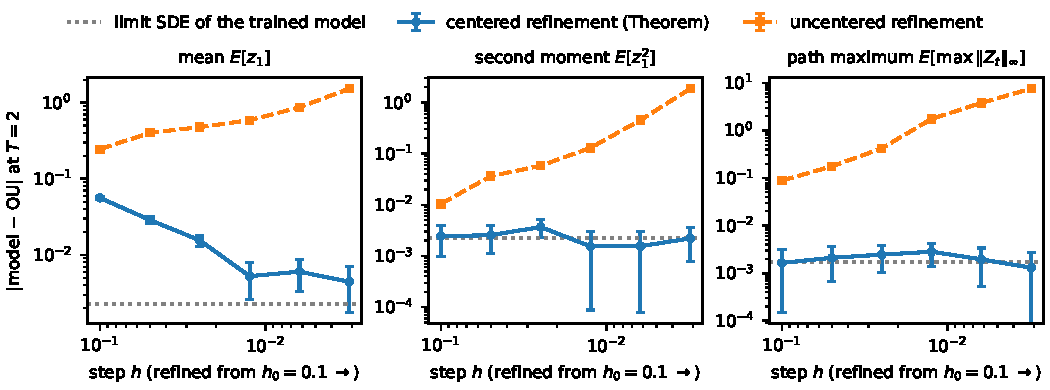
\includegraphics[width=\linewidth]{figures/weak_convergence_ou_row_print.pdf}
\caption{Centered refinement of a trained NormFlowSDE transition recovers a standard SDE. The reference process is the two-dimensional Ornstein--Uhlenbeck SDE $dZ=-KZ\,dt+S\,dW$ with $K=[1,\,0.8;\,-0.8,\,1]$, $S=[0.6,\,0;\,0.3,\,0.4]$ (rows separated by semicolons) and $Z_0=(2,-1)$. A NormFlowSDE model (drift network and conditional RealNVP noise flow, $\alpha=1.5$) was fitted by its exact one-step likelihood to transitions $z'=z-h_0Kz+\sqrt{h_0}\,S\eta$ at $h_0=0.1$, where $\eta$ has independent, skewed two-component-mixture coordinates with zero mean, unit variance and skewness $-0.38$. The finite-step increments are therefore non-Gaussian, while the only diffusion with the same first two moments is the reference process. With the fitted networks fixed, each panel shows the absolute error at $T=2$, relative to the exact Ornstein--Uhlenbeck law, of the mean of $z_1$, the second moment $z_1^2$, and the path maximum $\max_t\norm{Z_t}_\infty$ on the grid $t\in h_0\mathbb{N}$. The step decreases from $h_0$ to $h_0/32$ from left to right. Blue: the centered scheme of Theorem~\ref{thm:weak}, with $m_\phi$ and $A$ computed by $24\times24$ Gauss--Hermite quadrature. Orange: the uncentered refinement $z+hf_\varphi+\sqrt h\,g_\phi$. Dotted: the limit SDE of the fitted model, simulated by Euler--Maruyama at $h_0/128$; its distance to the reference process is the learning error that remains as $h\to0$. The fitted drift $b_{\rm eff}$ and diffusion $A$ differ from $-Kz$ and $SS^\top$ by at most $0.027$ and $0.0045$ on $[-2,2]^2$. The centered error of the mean decreases from $0.056$ at $h_0$, the bias of the coarse training chain, towards this learning-error floor; the other statistics are already near the floor at $h_0$. The fitted noise flow has a nonzero mean ($\norm{m_\phi}$ up to $0.83$), which is not identifiable from the drift in the trained update; without centering it acts as a drift of order $1/\sqrt h$, and the uncentered errors grow as $h$ decreases.}
\label{fig:weak-convergence-ou}
\end{figure}

\section{Derivation of the reconstruction and transition losses}\label{app:training-loss}

All densities below condition on the supplied initial state $z_0$, observations, and controls. The sequential generator has normalized path density
\begin{equation}\label{eq:training-path-density}
 q_\omega(\mathbf z)
 =\prod_{k=0}^{N-1}q_\omega(z_{k+1}\mid z_k,t_k,u_k,c_k).
\end{equation}
The fixed-scale Gaussian reconstruction model and the resulting auxiliary joint density are
\begin{align}
 p_\sigma(x_k\mid z_k)&=\N(x_k;z_k,\sigma_{\mathrm{state}}^2I_d),
 \qquad \sigma_{\mathrm{state}}>0,\label{eq:reconstruction-model}\\
 p_{\omega,\sigma}(\mathbf x,\mathbf z)
 &=q_\omega(\mathbf z)\prod_{k=1}^N p_\sigma(x_k\mid z_k).\label{eq:training-joint-density}
\end{align}
Expanding the expected negative joint log density gives
\begin{align}\label{eq:joint-training-loss}
 \mathcal L_{\mathrm{joint}}(\omega;\mathbf x)
 &=\E_{\mathbf z\sim q_\omega}[-\log p_{\omega,\sigma}(\mathbf x,\mathbf z)]\notag\\
 &=\E_{\mathbf z\sim q_\omega}
 \left[-\sum_{k=1}^N\log p_\sigma(x_k\mid z_k)
       -\sum_{k=0}^{N-1}\log q_\omega(z_{k+1}\mid z_k,t_k,u_k,c_k)\right]\notag\\
 &=\mathcal L_{\mathrm{state}}(\omega;\mathbf x)+\mathcal L_{\mathrm{trans}}(\omega).
\end{align}
The Gaussian reconstruction density yields Equation~\eqref{eq:state-training-loss}; its additive constant does not affect optimization at fixed $\sigma_{\mathrm{state}}$.

For a generated transition, the forward map from $\epsilon_k$ to $z_{k+1}$ has Jacobian $\sqrt{\Delta t}\,J_{\phi,k}(\epsilon_k)$. The change-of-variables identity in Equation~\eqref{eq:sampled-transition-density} therefore gives
\begin{align}\label{eq:self-transition-loss}
 \mathcal L_{\mathrm{trans}}(\omega)
 &=\E\left[\sum_{k=0}^{N-1}
 \left(-\log\N(\epsilon_k;0,I_d)+\log|\det J_{\phi,k}(\epsilon_k)|
       +\frac d2\log\Delta t\right)\right]\notag\\
 &=\E\left[\sum_{k=0}^{N-1}\log|\det J_{\phi,k}(\epsilon_k)|\right]
   +\frac{Nd}{2}\bigl[1+\log(2\pi\Delta t)\bigr].
\end{align}
The Gaussian term varies between sampled inputs, but its expectation is constant with respect to the trainable parameters. The remaining expected forward log determinant controls the path entropy.

\paragraph{Coupling-scale bound.}
Each affine coupling layer leaves one coordinate block unchanged and scales and shifts the other. Its log scales have the form $\alpha\tanh(\cdot)\in(-\alpha,\alpha)$, so each multiplicative scale lies in $(e^{-\alpha},e^\alpha)$. If layer $\ell$ transforms $d_\ell$ coordinates, its Jacobian is block triangular with an identity block and a diagonal block of those scales. Its log determinant is therefore the sum of the $d_\ell$ log scales and lies in $[-\alpha d_\ell,\alpha d_\ell]$. The shifts do not contribute to the determinant, and coordinate permutations have unit absolute determinant. Composing $L_{\mathrm f}$ layers gives $|\log|\det J_{\phi,k}(\epsilon)||\leq B=\alpha\sum_{\ell=1}^{L_{\mathrm f}} d_\ell$, uniformly over the input and conditioning variables; this is Equation~\eqref{eq:training-determinant-bound}. When the layers alternate between the two halves of an even-dimensional state, $\sum_\ell d_\ell=L_{\mathrm f}d/2$. The geometric mean of the singular values of $J_{\phi,k}$ then lies between $e^{-\alpha L_{\mathrm f}/2}$ and $e^{\alpha L_{\mathrm f}/2}$.

\paragraph{Entropy bound and noise floor.}
Equations~\eqref{eq:training-determinant-bound} and~\eqref{eq:self-transition-loss} imply
\begin{equation}\label{eq:transition-entropy-lower-bound}
 \mathcal L_{\mathrm{trans}}(\omega)
 \geq\frac{Nd}{2}\bigl[1+\log(2\pi\Delta t)\bigr]-NB.
\end{equation}
The entropy term is minimized by contraction, so wherever reconstruction does not oppose it, the bounded flow approaches this bound. The lower side of Equation~\eqref{eq:training-determinant-bound} then acts as a noise floor: the volume of the per-step increment $\sqrt{\Delta t}\,g_\phi$ cannot fall below $\Delta t^{d/2}e^{-B}$. The floor depends on $\alpha$ and $L_{\mathrm f}$ but not on the data. With two coupling layers and $\alpha=1$, for example, the geometric-mean noise scale cannot fall below $e^{-1}\approx0.37$.

\paragraph{Volume, not variance.}
Let $\sigma_1(\epsilon)\geq\cdots\geq\sigma_d(\epsilon)$ denote the singular values of $J_{\phi,k}(\epsilon)$. Equation~\eqref{eq:training-determinant-bound} constrains only their product, $|\det J_{\phi,k}(\epsilon)|=\prod_{i=1}^d\sigma_i(\epsilon)$, which is the local volume change of the map $\epsilon\mapsto g_\phi(\epsilon;z_k,t_k,u_k,c_k)$. It does not constrain the individual singular values. Thus, the bounded flow can reduce its local scale below $e^{-B/d}$ in some directions only by enlarging it in others. A per-coordinate factor that adds $\sum_i\log s_{\phi,i}$ to the log determinant, and thereby lowers the attainable volume itself, is required. 

\paragraph{Learned noise scale.}
In Equation~\eqref{eq:learned-noise-scale}, the factor $s_{\phi,i}>0$ multiplies coordinate $i$ of the bounded flow output, so the standard deviation of that coordinate of the increment is scaled by $s_{\phi,i}$. It is computed from the current state, time, control, and observation feature, so it can vary along a trajectory. To keep it positive and finite, we restrict its logarithm to a fixed interval $[a_-,a_+]$ with $a_-<0<a_+$, using a sigmoid of a network output $r_{\phi,i}$:
\begin{equation}\label{eq:learned-scale-parameterization}
 \log s_{\phi,i}=a_-+(a_+-a_-)\,\mathrm{sigmoid}\bigl(r_{\phi,i}+r_0\bigr),
 \qquad r_0=\log(-a_-/a_+).
\end{equation}
The offset $r_0$ is chosen so that a network output of zero gives $s_{\phi,i}=1$, that is, no change to the flow. 

\paragraph{Effect on the bounds.}
Scaling coordinate $i$ by $s_{\phi,i}$ multiplies the volume by $s_{\phi,i}$, so the log determinant gains $\sum_i\log s_{\phi,i}$. This sum lies in $[d\,a_-,\,d\,a_+]$, and the bounded flow contributes a value in $[-B,B]$. Equation~\eqref{eq:training-determinant-bound} therefore still holds, with the lower exponent widened to $B_-=B+d\,|a_-|$ and the upper exponent to $B_+=B+d\,a_+$. Likewise, the entropy lower bound~\eqref{eq:transition-entropy-lower-bound} holds with $B$ replaced by $B_-$, which is $d\,|a_-|=10d$ lower per transition.

\paragraph{Why a proper score is needed.}
Because the entropy term rewards contraction, the much lower bound means that this term alone could shrink the noise almost to zero. The learned scale is therefore trained with an objective that also penalizes too little spread, such as the full-horizon energy score of Section~\ref{sec:training-rollout}. The energy score is a proper scoring rule: it is smallest when the generated spread matches the true conditional spread, whether that spread is large or small. With the bounded flow alone, a true spread below the floor cannot be reached. The learned scale makes it reachable.

Finally, the transition term equals $H(q_\omega)=\E_{q_\omega}[-\log q_\omega]$, giving
\begin{equation}\label{eq:joint-training-loss-entropy}
 \mathcal L_{\mathrm{joint}}(\omega;\mathbf x)
 =\mathcal L_{\mathrm{state}}(\omega;\mathbf x)+H(q_\omega).
\end{equation}
The marginal reference-state NLL, $-\log\int p_{\omega,\sigma}(\mathbf x,\mathbf z)\,d\mathbf z$, integrates out the generated path and is a different objective. If $q_\omega$ is used as the variational path density for the auxiliary model, the negative ELBO cancels the transition entropy:
\begin{equation}\label{eq:joint-versus-elbo}
 \begin{aligned}
 \E_{\mathbf z\sim q_\omega}
 \left[-\log p_{\omega,\sigma}(\mathbf x,\mathbf z)+\log q_\omega(\mathbf z)\right]
 &=\mathcal L_{\mathrm{state}}(\omega;\mathbf x)+H(q_\omega)-H(q_\omega)\\
 &=\mathcal L_{\mathrm{state}}(\omega;\mathbf x).
 \end{aligned}
\end{equation}
The proposed composite objective retains the entropy penalty.

\section{Implementation and reproducibility details}\label{app:reproducibility}
This appendix summarizes the details about data generation, methods training and evaluation for reproducinf the results in Section~\ref{sec:experiments}.

\subsection{Data generation}\label{app:data}
Each dataset is a cache of fixed-length windows, each with a known initial state, a control sequence, noisy observations, and the reference states used for training and scoring. The data are split by trajectory or episode before windowing, and normalization statistics are computed on the training split only; pendulum and Lorenz--96 metrics are reported in physical units. The observation noise of Equation~\eqref{eq:obsnoise} is drawn independently for every observed coordinate and time step.The caches are rebuilt deterministically from fixed seeds and were verified against stored checksums before training.

\paragraph{Pendulum.}
320 trajectories of 60 steps follow Equation~\eqref{eq:pendulum} with $g=9.81$, $\ell=m=1$, $c=0.2$, $\sigma_\theta=0.01$, $\sigma_\omega=0.2$, integrated by Euler--Maruyama with eight substeps per interval $\Delta t=0.05$. The torque is a smooth, bounded random signal, $u_k=3\tanh(r_k)$ with $r_k$ a first-order autoregressive process. The angle is unwrapped. Each trajectory is one window; the split is 224 / 48 / 48 and the noise scale is $\sigma=0.1$.

\paragraph{Lorenz--96.}
2000 independent trajectories of Equation~\eqref{eq:lorenz96} ($d=12$, $F=8$, RK4 at $\Delta t=0.02$) start from a small random perturbation of the origin and are integrated for 500 spin-up steps; the next 100 steps form the window and the state at the end of the spin-up is the known initial state. Every second coordinate is observed with $\sigma=0.5$. The split is 1600 / 200 / 200 trajectories, of which the first 100 test windows are scored.

\paragraph{ALOHA insertion.}
The 50 teleoperation episodes of the simulated bimanual insertion task \citep{zhao2023aloha} at 50\,Hz are split 40 / 5 / 5. The 14 commanded joint positions are the controls and the 14 measured follower-joint positions, perturbed as described in Appendix~\ref{app:aloha-disturbance}, are the states. Windows of 250 steps are cut with a stride of 25 frames, giving 400 / 50 / 50 windows. States and controls are normalized per joint, and the noise ($\sigma=0.1$) is added in normalized units.

\paragraph{REASSEMBLE.}
The 148 episodes of the 30\,Hz real-robot dataset \citep{sliwowski2025reassemble} are split 94 / 17 / 37. The state is the seven joint positions and the nine-dimensional command is the control. Windows of 250 steps are cut without overlap; the training split is capped at 2000 windows, and 300 windows each are used for validation and test. Normalization and noise are as for ALOHA.

\subsection{ALOHA latent disturbance}\label{app:aloha-disturbance}
The recorded ALOHA states are deterministic given the commands, so we add a slowly varying latent disturbance per episode in joint-position units before normalization. With $q_k$ the recorded joint positions and $u_k$ the commands,
\begin{equation}\label{eq:alohadisturbance}
 \tilde q_{k+1}=\tilde q_k+(q_{k+1}-q_k)+\Delta t\,B\,d_k,\qquad
 d_{k+1}=\rho\,d_k+\sigma_d\,(1+\gamma\,r_k)\,\xi_k,\qquad \xi_k\sim\N(0,I_4),
\end{equation}
starting from $\tilde q_0=q_0$ and $d_0=0$, with $\rho=0.98$, $\sigma_d=0.05$, $\gamma=2$, $\Delta t=0.02$, and $B=0.35\,Q$ for a fixed random orthonormal $14\times4$ matrix $Q$. The regime variable $r_k$ is the command-tracking error of the frame relative to its median over the training episodes, capped at 3, so that the disturbance grows during contact. The disturbed trajectory $\tilde q$ is the reference state; the commands are unchanged; the observation of $\tilde q_{k+1}$ adds the noise of Equation~\eqref{eq:obsnoise}.

\subsection{Evaluation protocol}\label{app:protocol}
All methods filter causally from the known initial state and never see future observations or intermediate reference states. For every test window a method returns $M$ posterior draws per time step ($M=128$, 200, 200, 500 on the pendulum, Lorenz--96, ALOHA, and REASSEMBLE); the particle filters run with the protocol particle count (500, 1000, 200, 500) and return $M$ draws from the weighted particles. RMSE is computed per window and averaged over windows; CRPS is the empirical marginal CRPS of the draws, averaged over windows, steps, and coordinates; the energy score is computed on the state vector at each step; coverage is the fraction of reference values inside the central interval between the empirical quantiles of the draws, pooled over windows, steps, and coordinates, and width is the mean length of that interval. Every method is trained with three seeds on the same caches and with the same total number of optimizer updates per dataset (8400, 18500, 9000, 11000, the largest of the four methods' tuned recipes). Checkpoints and hyperparameters are selected on the validation split, by the lowest validation RMSE unless stated otherwise, and no post-hoc calibration is applied. Tables report the mean and sample standard deviation over the three seeds.

\subsection{\method}\label{app:normflowsde}
\paragraph{Architecture.}
The drift and the conditional RealNVP noise flow receive the state, the window feature, and, where available, the control. The encoder is a bidirectional GRU that reads only the last $o=10$ measurements, each concatenated with its control (the window feature of Equation~\eqref{eq:sequence-conditioning}). Table~\ref{tab:nfsde-arch} lists the sizes; the parameter counts of all methods are in Table~\ref{tab:params}.
\begin{table}[htbp]
\centering\footnotesize
\begin{tabular}{lcccc}
\toprule
 & Pendulum & Lorenz--96 & ALOHA & REASSEMBLE \\
\midrule
Window feature $d_c$ / encoder width & 16 / 16 & 128 / 128 & 64 / 64 & 64 / 64 \\
Drift width / depth & 88 / 2 & 256 / 3 & 128 / 3 & 128 / 3 \\
Coupling layers / coupling width & 6 / 88 & 2 / 64 & 2 / 64 & 2 / 64 \\
Log-scale bound $\alpha$ (stage 1 / 2) & 1 / 1 & 1.5 / 1.5 & 1 / 1 & 1 / 2 \\
Sampler & Euler & Heun & Euler & Euler \\
\bottomrule
\end{tabular}
\caption{\method architecture per dataset. ``Heun'' is a stochastic predictor--corrector step that reuses one Gaussian draw at the predicted and corrected states.}
\label{tab:nfsde-arch}
\end{table}

\paragraph{Stage 1: composite objective.}
The first stage minimizes the objective of Equation~\eqref{eq:normflowsde_loss} on random training windows with the multiple-shooting partition of Section~\ref{sec:training}, using a bounded flow without the learned scale. Table~\ref{tab:nfsde-stage1} lists the dataset-specific settings. Four generated trajectories per window enter the state and transition terms; the rollout term is the energy score of Equation~\eqref{eq:energy-score-estimator} over the full window, evaluated every few updates with the stated number of draws. The optimizer is AdamW with gradient clipping. Lorenz--96 uses a warm-up and cosine learning-rate schedule, epoch-wise shuffling, and a small auxiliary one-step likelihood term; the other datasets use a constant learning rate. The checkpoint with the lowest validation RMSE initializes the second stage.
\begin{table}[htbp]
\centering\footnotesize
\begin{tabular}{lcccc}
\toprule
 & Pendulum & Lorenz--96 & ALOHA & REASSEMBLE \\
\midrule
Updates & 4400 & 14500 & 5000 & 7000 \\
Trajectories per update & 16 & 64 & 1 & 4 \\
Learning rate & $6\times10^{-4}$ & $2\times10^{-3}$ & $3\times10^{-4}$ & $10^{-3}$ \\
Segment length (states) & 11 & 5 & 5 & 5 \\
$\sigma_{\mathrm{state}}$ (normalized units) & 1 & $1/\sqrt2$ & 1 & 1 \\
$\lambda_{\mathrm{cont}}$ & 1 & 0.1 & 1 & 1 \\
$\lambda_{\mathrm{rollout}}$ / rollout draws & 30 / 4 & 1 / 8 & 0 / -- & 0.5 / 4 \\
\bottomrule
\end{tabular}
\caption{Stage-1 settings of \method. On ALOHA the rollout term is switched off in stage 1 and enters only through stage 2.}
\label{tab:nfsde-stage1}
\end{table}

\paragraph{Stage 2: full-horizon energy score with the learned scale.}
The second stage warm-starts from the stage-1 checkpoint and adds the learned per-coordinate scale of Equation~\eqref{eq:learned-noise-scale}, initialized so that the model is unchanged at the first step. It minimizes the energy score of Equation~\eqref{eq:energy-score-estimator} of $M=16$ complete filtering rollouts per window, generated exactly as at inference, for 4000 updates on batches of 16 windows with a warm-up and cosine schedule (learning rates $3\times10^{-3}$, $3\times10^{-5}$, $3\times10^{-4}$, and $10^{-4}$ on the four datasets). The selected checkpoint has the lowest validation RMSE, except on Lorenz--96 where it has the lowest validation CRPS. On REASSEMBLE the coupling log-scale bound is raised to $\alpha=2$ and the weight of the pairwise spread term in Equation~\eqref{eq:energy-score-estimator} is 0.52 instead of $1/2$; the latter slightly rewards dispersion, so the width of the REASSEMBLE intervals should be read with this in mind.

\paragraph{Hyperparameter selection.}
The ALOHA configuration was selected inside the benchmark campaign by validation RMSE. The pendulum, Lorenz--96, and REASSEMBLE configurations come from small follow-up sweeps with the same budgets, caches, seeds, and selection metric, over the stage-1 rollout weight, reconstruction scale, batch size, and learning rate, and over the stage-2 learning rate, bound $\alpha$, spread weight, and selection metric. Among configurations whose validation RMSE was within noise of each other, the one whose validation coverage was closest to nominal was kept and trained for all three seeds. The sweep runs computed test metrics at the end of each run, so the test split was visible during these rounds; the reported numbers are those of the selected configuration's three seeds.

\subsection{Particle-filter baselines}\label{app:baselines}
The widths of all baselines were chosen so that each method's parameter count matches \method per dataset as closely as its architecture allows (Table~\ref{tab:params}).
\begin{table}[htbp]
\centering\footnotesize
\begin{tabular}{lcccc}
\toprule
Parameters ($\times10^3$) & Pendulum & Lorenz--96 & ALOHA & REASSEMBLE \\
\midrule
\method (stage 1 / stage 2) & 91.0 / 103.6 & 349.3 / 365.4 & 116.6 / 129.7 & 108.6 / 120.4 \\
NF-DPF & 92.4 & 351.2 & 116.3 & 108.8 \\
NSF-PF & 64.1 & 144.6 & 80.5 & 68.4 \\
FlowSDE-PF & 110.2 & 279.4 & 126.7 & 111.0 \\
\bottomrule
\end{tabular}
\caption{Parameter counts of the selected models. The stage-2 count of \method includes the learned-scale network.}
\label{tab:params}
\end{table}

\paragraph{NF-DPF.}
Our implementation of \citet{chen2025flowparticle} has a conditional-RealNVP transition, an observation-conditioned proposal flow, and a conditional-RealNVP measurement density, with importance weights that include the transition and proposal densities. Training has two stages. The first trains on short 8-step windows with 32 particles and differentiable optimal-transport resampling, starting with the supervised likelihoods of the three components and then switching to the end-to-end filtering error. The second warm-starts the best stage-1 checkpoint and trains on a curriculum of increasing horizons up to the full window with 64 particles, minimizing the weighted-particle CRPS together with the measurement likelihood. At test time the filter runs with the protocol particle count and systematic resampling.

\paragraph{NSF-PF and FlowSDE-PF.}
The transition is the exact-density Neural Stochastic Flow of \citet{kiyohara2025nsf} or a FlowSDE drift \citep{lou2026flowsde} with fixed isotropic diffusion trained by bridge flow matching and integrated by Euler--Maruyama with four substeps per interval; both condition on the control and the time but not on observations. The measurement density $q(y\mid x)$ is a conditional RealNVP with four coupling layers. Dynamics and measurement flow are trained jointly by maximum likelihood on random training windows for the full update budget. During training, a bootstrap particle filter is run on the validation windows at regular intervals, and the checkpoint and a process-noise inflation (an isotropic Gaussian jitter added to every predicted particle, chosen from a fixed grid) are selected jointly by validation RMSE. FlowSDE is additionally trained for three diffusion levels, selected the same way.

\subsection{Model-based reference filters}\label{app:references}
On the pendulum and Lorenz--96 the data-generating model is known. The EKF and UKF use the true dynamics with the moment-matched Gaussian likelihood of the mixture; the bootstrap particle filter uses the true dynamics with the exact mixture likelihood and the protocol particle count. The process-noise scale of each filter is selected on the validation windows from a small grid, and the smallest grid value was selected in every case. Three filter seeds are run on the same caches as the learned methods.

\subsection{Latency, calibration curves, and noise recovery}\label{app:analyses}
\paragraph{Latency.}
Each method's selected seed-0 checkpoint filters single test windows on one NVIDIA L40S. The first call, which compiles, is excluded, and the median over 30 further calls on different test windows is reported. \method runs with the protocol $M$, the particle filters with the protocol particle count. The reference filters are timed with the same procedure.

\paragraph{Calibration curves.}
Figure~\ref{fig:calibration} evaluates the coverage of central intervals at nominal levels from 10\% to 95\% from the saved test posteriors of all three seeds, pooled over windows, steps, and coordinates; the curves show the seed mean and the shading the seed range.

\paragraph{Noise recovery.}
Figure~\ref{fig:noise-recovery} uses the seed-0 runs. For each particle filter the learned measurement flow is evaluated on one-coordinate slices around 100 random test states and averaged over states and coordinates; its total-variation distance to the mixture is computed on the same grid. The implied residuals $y-\E[x\mid y]$ use the posterior mean on all test windows. For the pendulum and Lorenz--96, residuals are rescaled to the physical units in which the noise is defined.

\subsection{Software, hardware, and code availability}\label{app:scripts}
All models are implemented in JAX 0.10 with Equinox 0.13 and Optax 0.2 under Python 3.12. Training ran on NVIDIA A100 GPUs of a university cluster and on local A30 and RTX Pro 6000 GPUs; the latency measurements ran on a dedicated L40S. The code, the manuscript, and the frozen run directories are available at \url{https://github.com/papersubmit-a/NormFlowSDE}; the layout of the archive and the commands that rebuild the tables and figures are documented in its \path{README.md}. The code is released under the MIT License. The posterior and data arrays are too large for the repository and are not yet approved for redistribution; this draft makes no public-availability promise for them.

\end{document}
